\documentclass[10pt]{article}
\usepackage{outlines}
\usepackage{amssymb}
\usepackage{amsmath}
\usepackage{graphicx} % Required for inserting images
\usepackage[a4paper, margin=2.5cm]{geometry}
\usepackage{eso-pic}
\usepackage{tikz}
\AddToShipoutPictureBG{%
  \begin{tikzpicture}[remember picture,overlay]
    \draw[line width=1pt] 
      ([xshift=2cm,yshift=-2cm]current page.north west) 
      rectangle 
      ([xshift=-2cm,yshift=2cm]current page.south east);
  \end{tikzpicture}%
}
\usepackage{wrapfig}
\usepackage{float}  % In preamble

\usepackage[
backend=biber,
style=apa,
]{biblatex}
\addbibresource{main.bib} %Imports bibliography file

\usepackage{setspace}
\doublespacing
\newcommand{\specialcell}[2][c]{%
  \begin{tabular}[#1]{@{}c@{}}#2\end{tabular}}

\begin{document}
\pagenumbering{gobble} 
\begin{titlepage}
    \centering
    \vspace*{\fill}
    
    {\Large \textbf{An Investigation Into the Optimisation of Potting a Coin in Carromboard}}

    \vspace{2cm}
    
    {\Large By Gautam Bansal}
    
    \vspace{2cm}
    
    \begin{abstract}
    \noindent This investigation explores how direct and glancing collisions in the board game carrom can be
mathematically modelled to find the optimum striker angle and placement to pot a coin. To achieve
this, two methods are developed. First, a purely geometric function is found that evaluates angular deviation by assuming fully elastic collisions and ignoring friction. With numerical
partial differentiation and Hessian matrices, this model is mathematically optimised to find critical
points that represent the best possible striker shots with zero angular deviation. Then, a kinematic function that considers friction, initial velocity, and masses is derived to accurately calculate the coin’s
final stopping distance to the pot. This physics-based approach is then numerically optimised through by programatically generating comprehensive heatmaps showing coin “pottability”
across the board. Together, these methods demonstrate how differentiatial calculus can balance mathematical complexity with tractability, effectively optimizing real-world strategies.
    \end{abstract}
    
    \vspace*{\fill}
\end{titlepage}

\pagebreak
\tableofcontents
\pagebreak

\pagenumbering{arabic} 
\setcounter{page}{1}
\section{Introduction}
       
\subsection{Background}
Multivariable calculus and differentiation, including the Hessian matrix, may be used to efficiently model and solve numerous real-world optimization problems. To explore this practically, this paper investigates the mechanics and optimization of potting a coin in the board game carrom, as it involves various components such as friction, collisions, both direct and glancing, and angles. By focusing through a mathematical lens with the help of relevant physics, and involving calculus, developing functions, and performing optimization, an effective answer may be gained to the question: \textbf{What is the optimum striker angle and placement for a striker to optimally pot a coin in carrom?}

\subsection{Modelling Functions}
To start with, it will be required to model functions regarding coins being potted, with the involvement of angles, velocities, placements, and collisions, and then eventually  mathematically obtaining such a function that can be optimised with the help of differential calculus and Hessian matrices.
\subsubsection{Assumptions}
To successfully model the carromboard, various assumptions must be made. Figure \ref{fig:realCarrom} demonstrates the realistic initial setup for carrom with a 7-coin setup.

\begin{figure}[h]
    \centering
    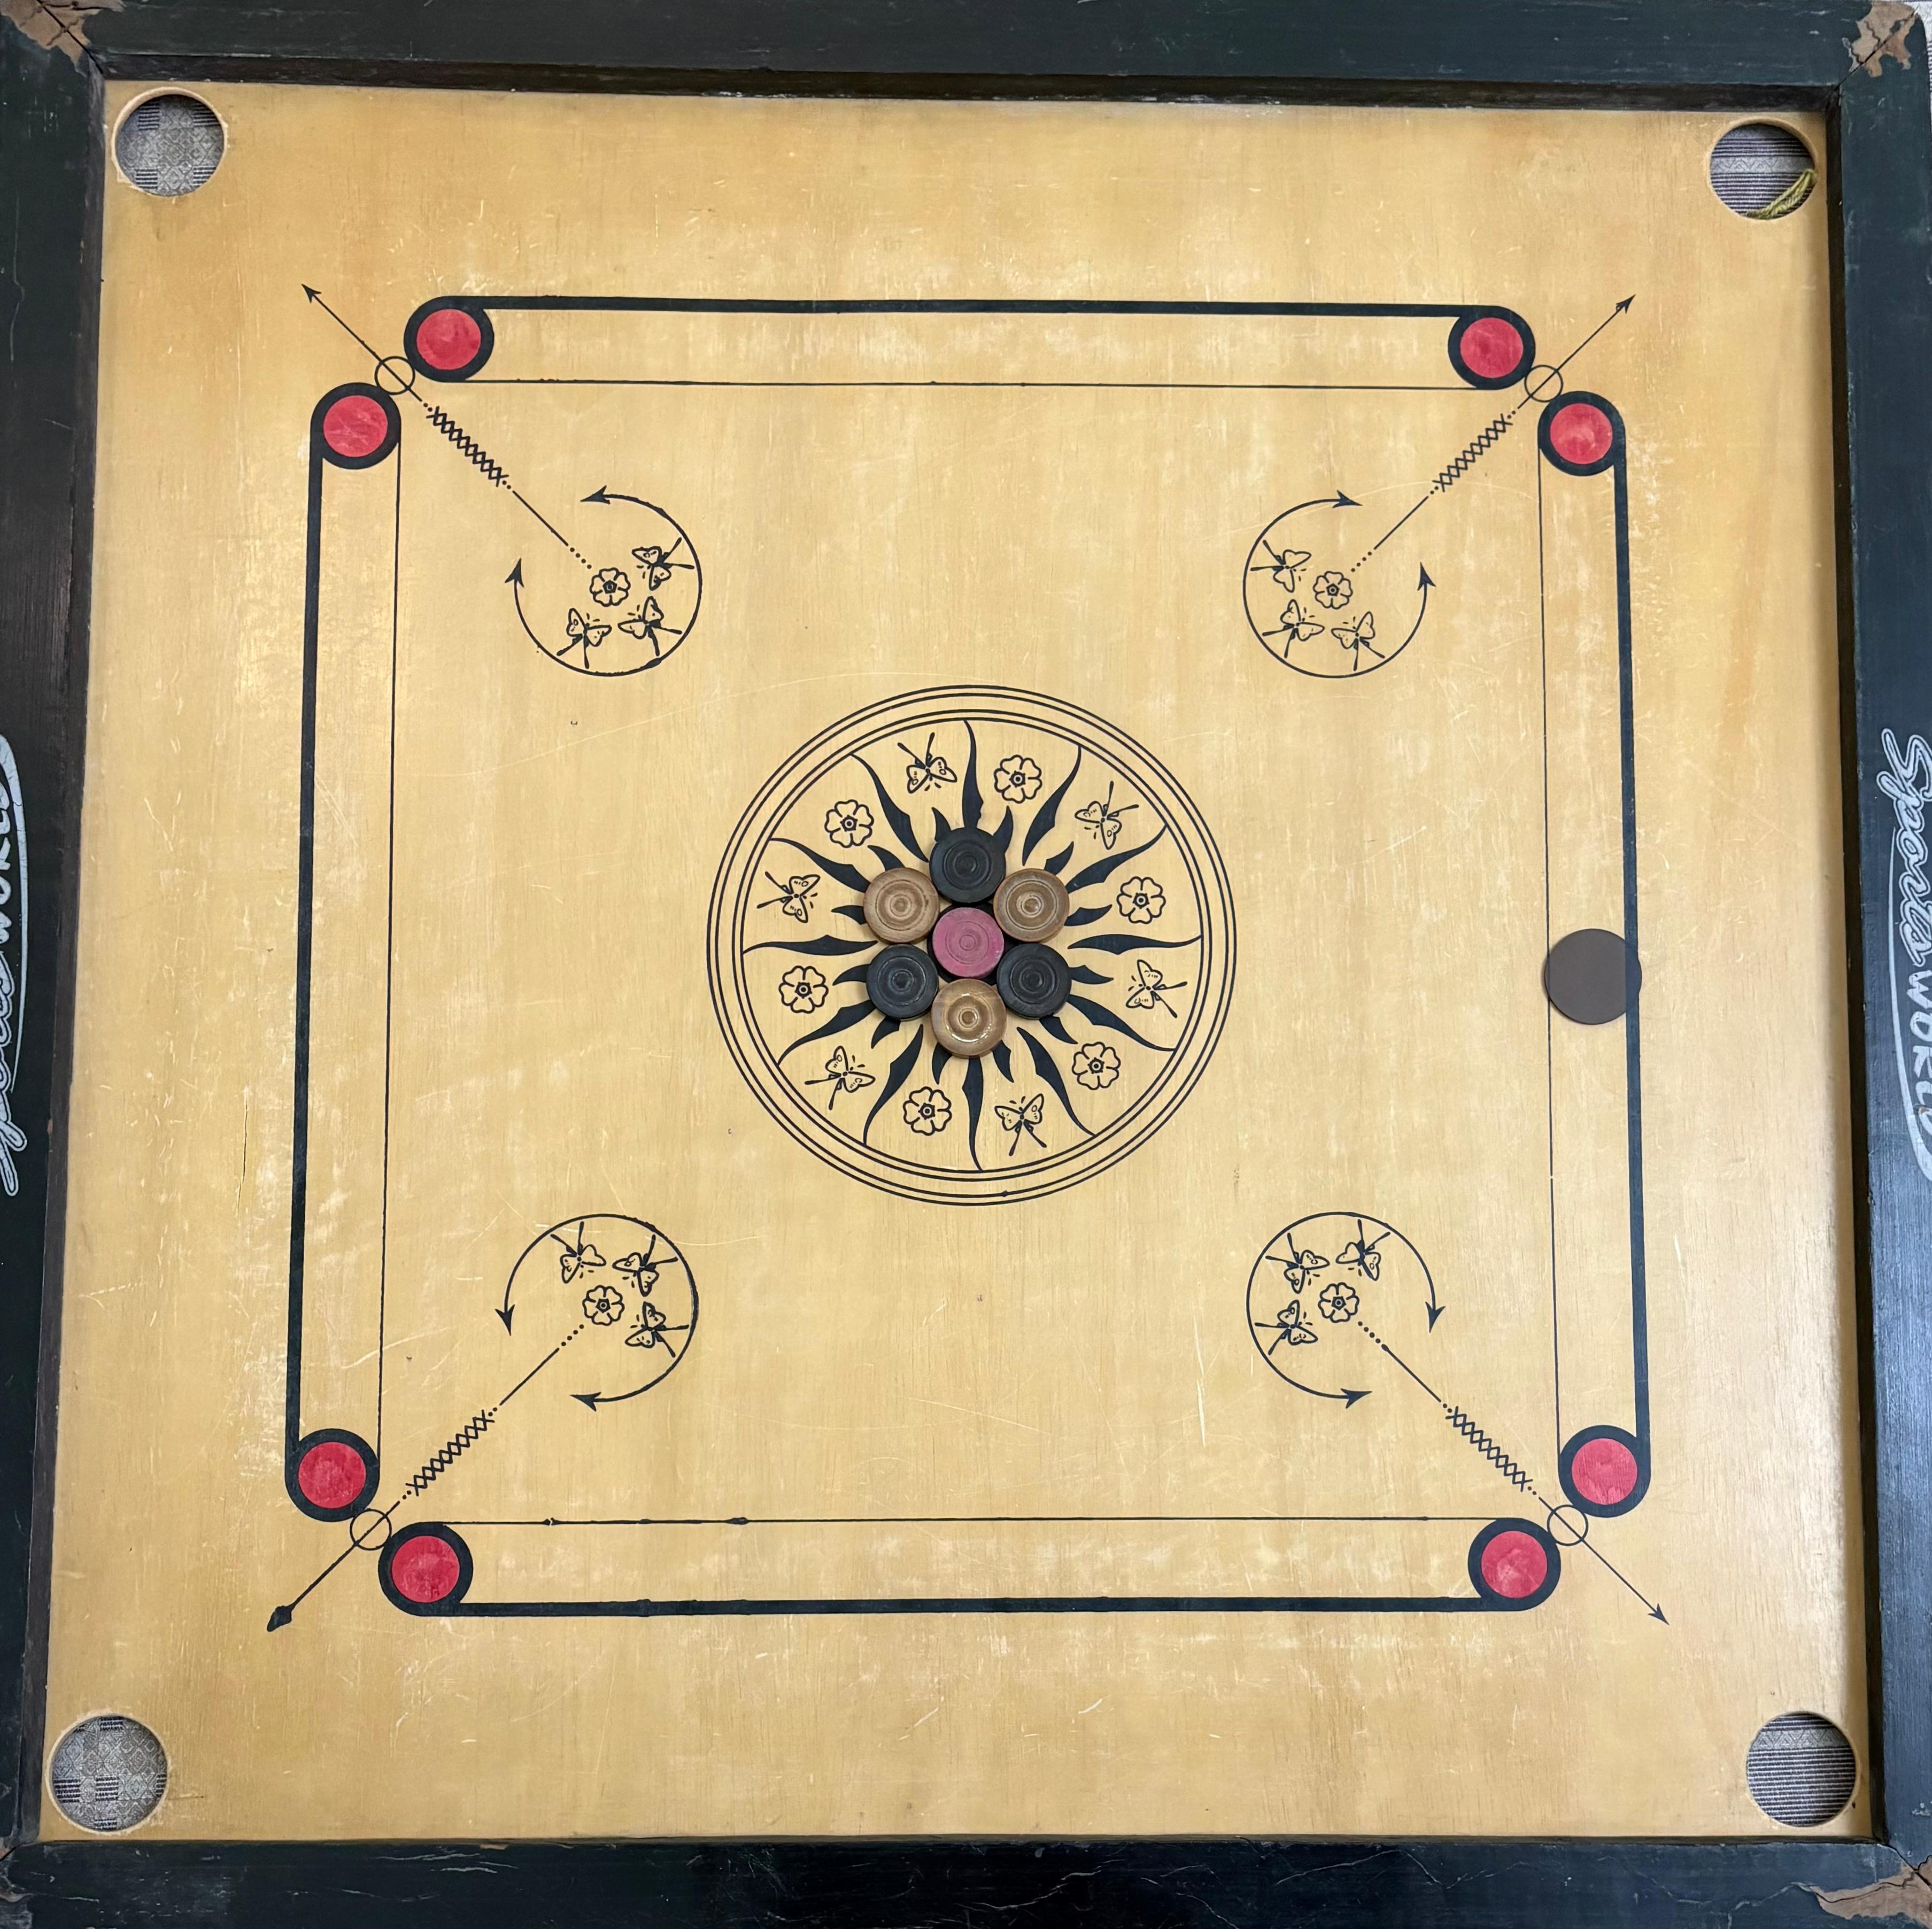
\includegraphics[width=0.3\linewidth]{Carromboard.png}
    \caption{Realistic Initial Setup of 7-coin carrom}
    \label{fig:realCarrom}
\end{figure}

The first assumption is that the board is uniform, meaning friction is uniform across the board. In reality, this is not true and friction may even be different across the board in each game due to the manual application of boric acid for reducing friction.

Secondly, collisions are elastic and occur on a 2D plane -- this means any 'ups' or 'downs' of the board, along with heights of coins, will not have a significant impact, and collisions will have complete transfers of kinetic energy which, though unrealistic, allows for a complete and thorough investigation.

Coins and strikers will be modelled to have equal rigid masses, and glancing collisions will be modelled as they are vital in carrom, but spin and rotation will not be as they are rarer especially among amateur players, and would result in too many factors to consider.

Secondary effects such as multiple rebounds involving the board's walls introduce a level of computational complexity beyond the scope of this exploration. To maintain mathematical tractability, such rebounds will hence be excluded.

The functions will also be modelled with knowing the dimensions of a standard Sports World carromboard along with the coins and striker, as shown in Figure \ref{fig:dim} to limit function inputs and allow for exact results. It is expected that though various assumptions will have to be made, results will match real patterns closely, as the vital factors such as friction and glancing collisions will be considered.

\begin{figure}[h]
    \centering
    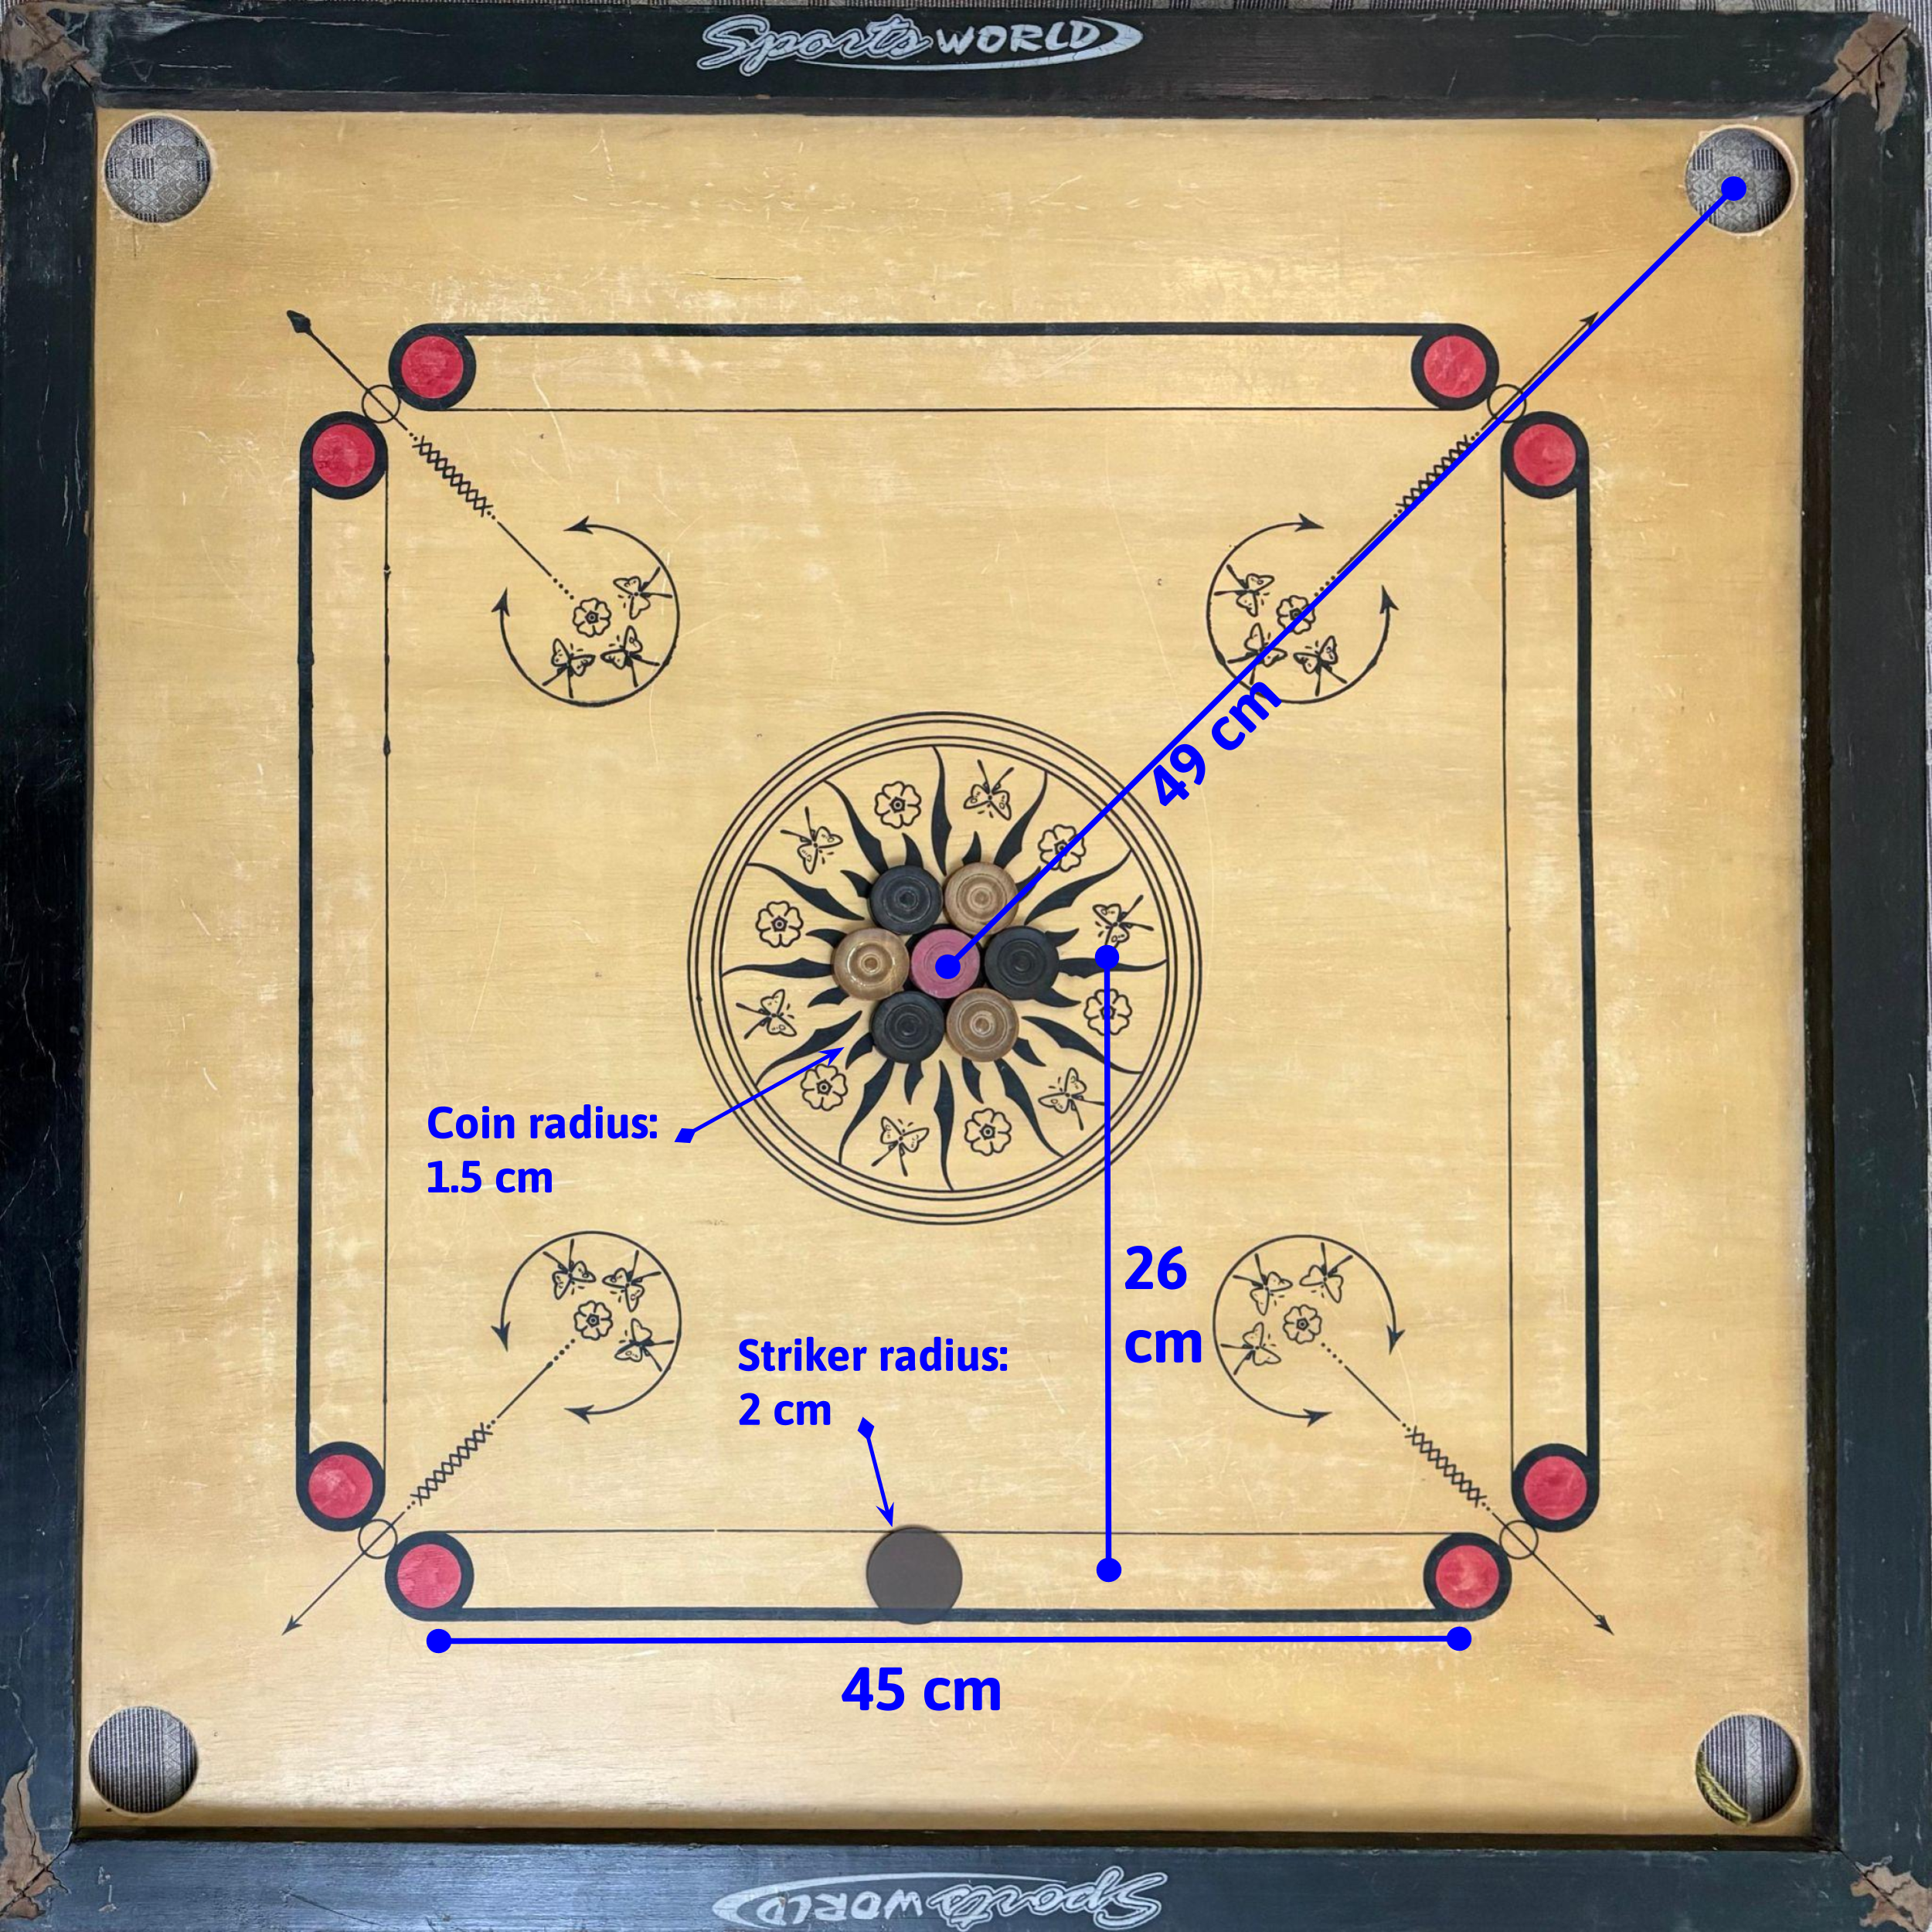
\includegraphics[width=0.4\linewidth]{Carrom-Dimensions.png}
    \caption{Dimensions of Sports World Carromboard And Pieces}
    \label{fig:dim}
\end{figure}            

Along with these measures of length, a few factors to consider include that striker mass is approximately 5 grams, coin mass is 7 grams, and striker velocity can approximate 120-200 centimeters per second, but a fairly normal striker shot would be approximately 170 centimeters per second. 

\subsection{Aim}
As such, the aim of this analysis is to explore how mathematically collisions and glancing collisions in carromboard can be modelled. The limitations and advantages of these methods will be carefully investigated, with the help of calculus and differentiation to optimise and find optimal striker positioning and striking as well.

\subsection{Methodology}
First a function will be derived that considers simply the angular deviation and ignores both friction and masses, considering fully elastic collisions, and assuming that if hit with the right velocity if the angular deviation of this function is 0 or near 0, it is possible to get the coin in. It will also consider both pots.

Secondly, a function that considers friction, velocity, and masses will be derived which will accurately provide an angular deviation to the closer pot. 

Finally, Hessian matrices and partial differentiation will be used for optimising these functions to discover the easiest and best carrom shots along with discovering what coins are impossible to get in directly.

\section{Method 1: Purely Mathematical and Geometric Model}

For the purposes of this method, a function that inputs angle of striker shot ($\theta$), striker x-coordinate ($x_s$), coin x-coordinate ($x_c$), and coin y-coordinate $y_c$ will be developed and derived, outputting the expected angular deviation. There will also be a condition to ensure the striker collides with the coin. Constraints on each of these inputs will also ensure the function works as expected realistically.

\subsection{Constraints and Situation Regarding Function Inputs}

To develop a proper function, first a 2D Cartesian coordinate plane will be developed using the carromboard, in which each unit is 1 centimeter. The x-axis will be set at the baseline where the striker is shot from, while the y-axis will cut through the centre. Each input variable will have constraints to ensure it is realistic, developed based on the carromboard's dimensions, as shown in Figure \ref{fig:m1const}.

\begin{figure}[h]
    \centering
    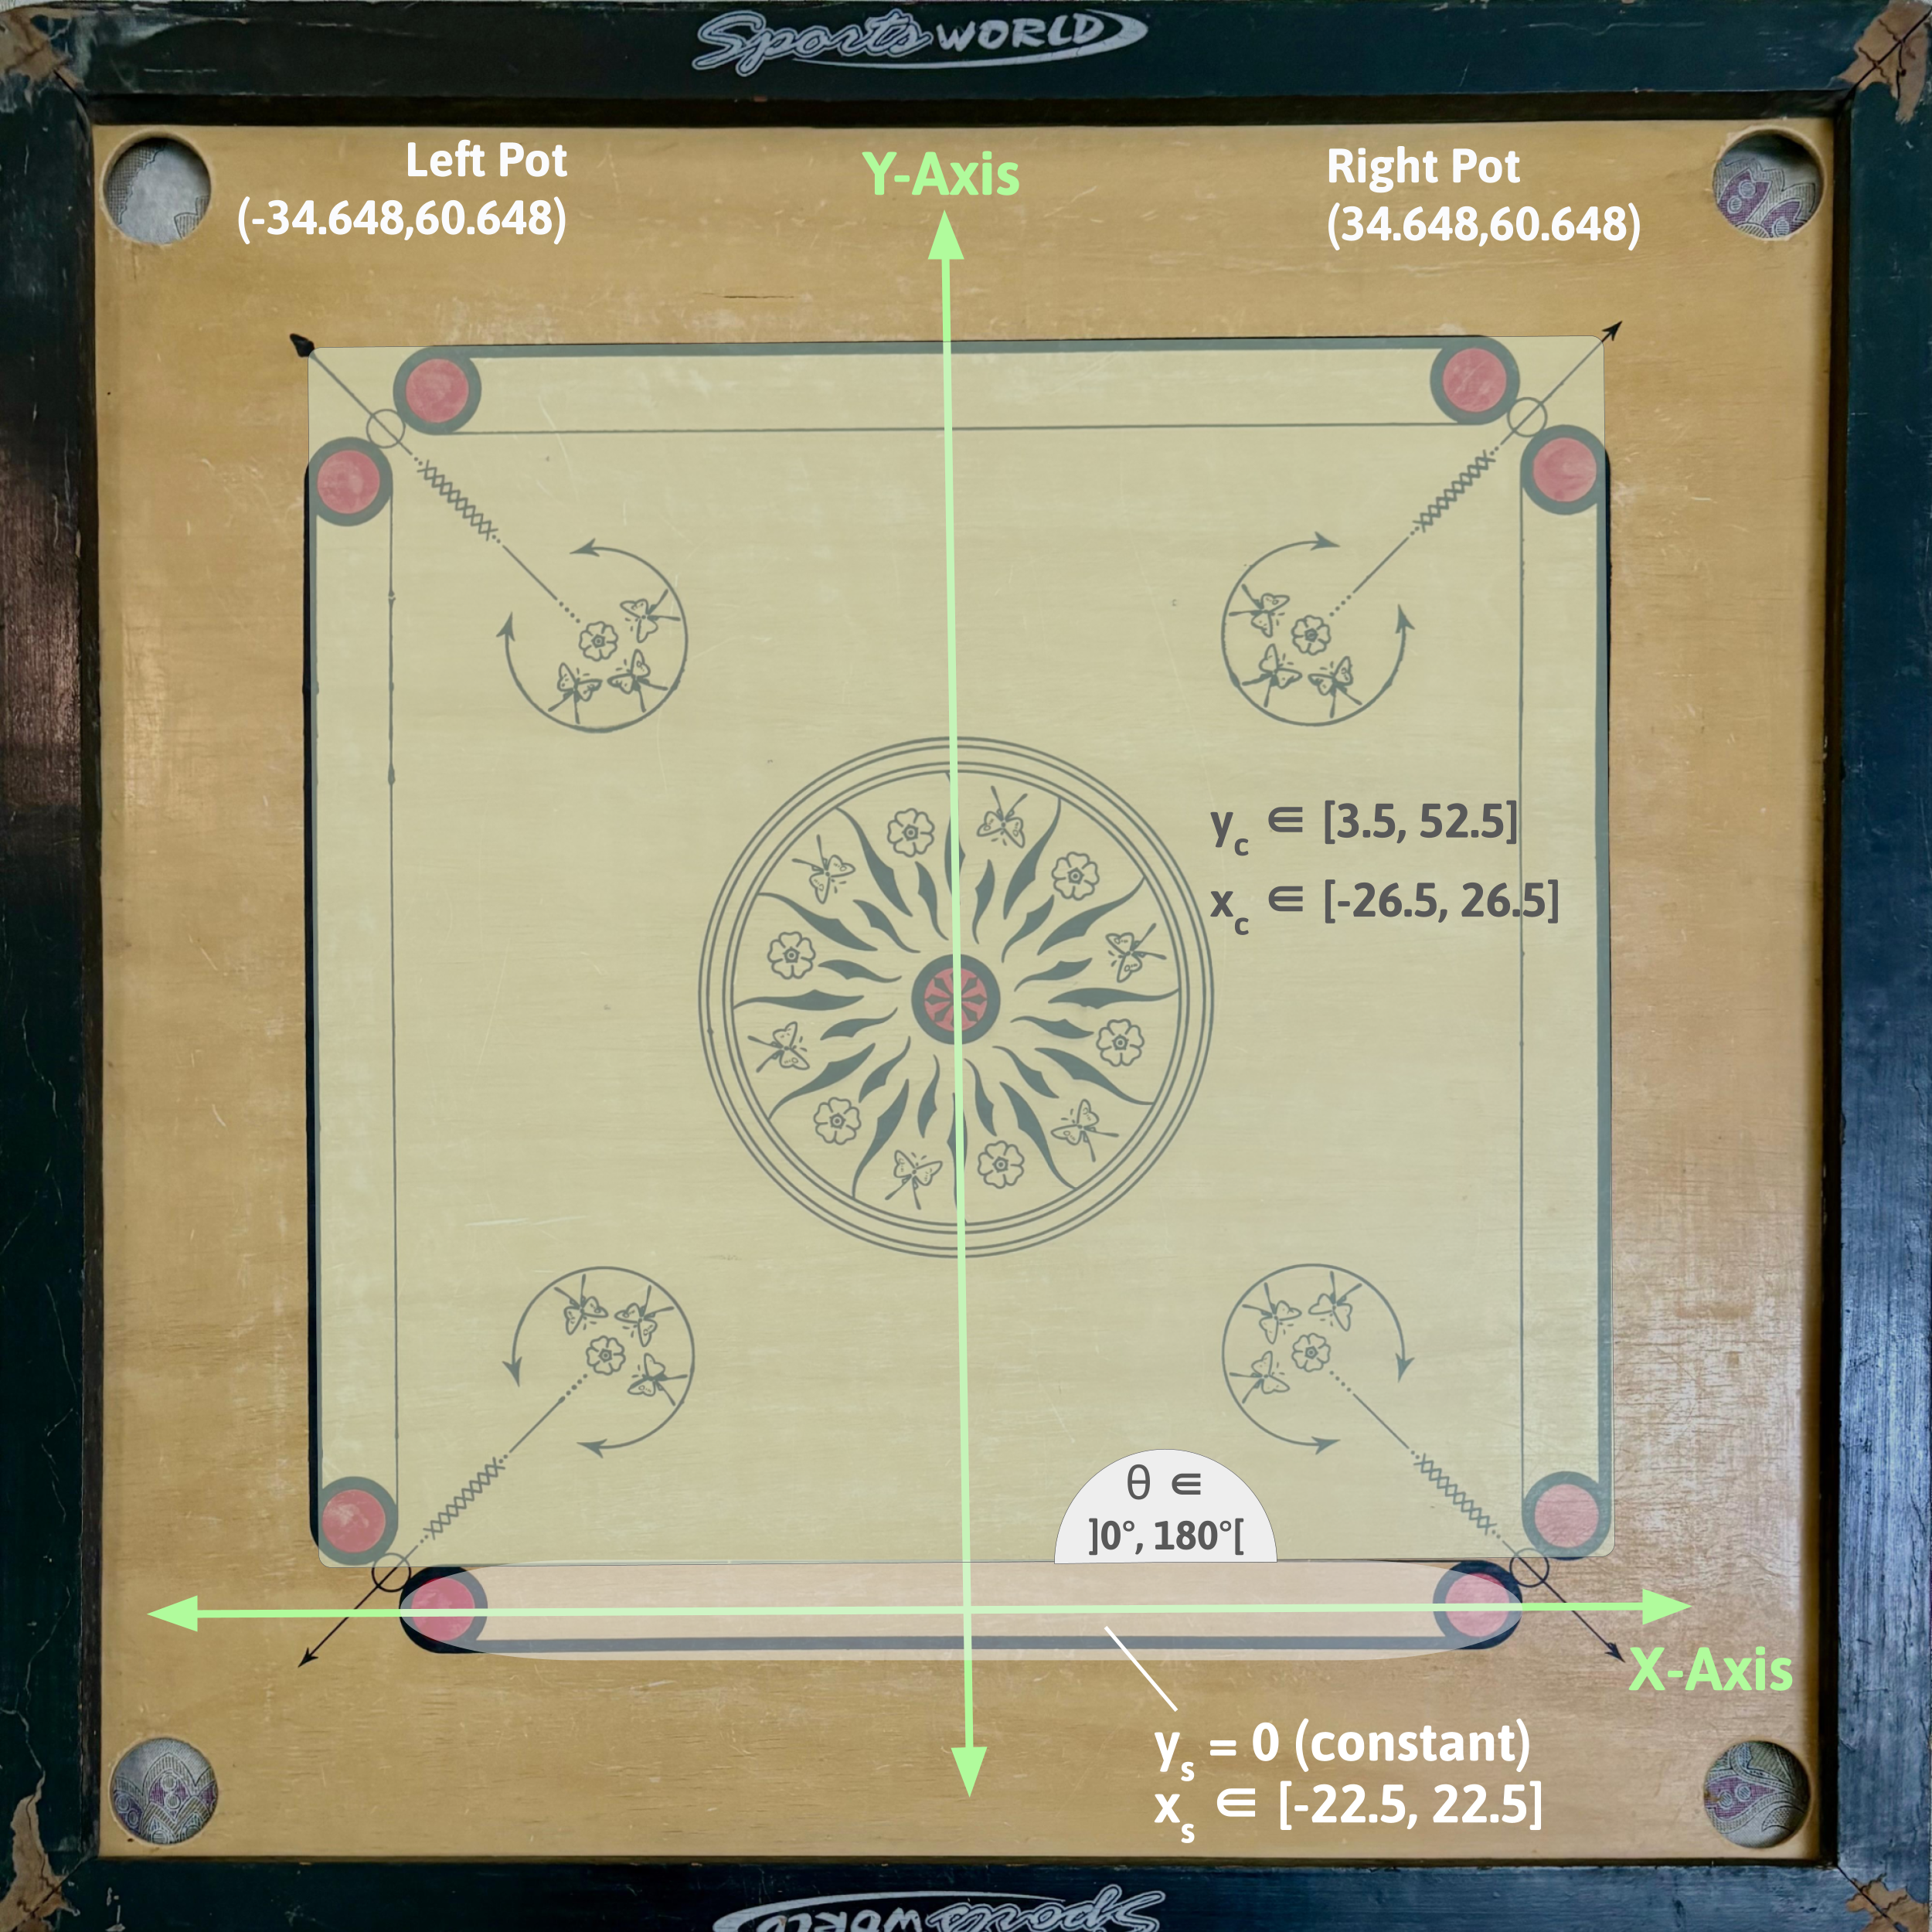
\includegraphics[width=0.5\linewidth]{CarromM1Inputs.png}
    \caption{Constraints on Each Input in Cartesian Carromboard Coordinate Plane}
    \label{fig:m1const}
\end{figure}

\subsection{Collision Condition}
Let us first develop an expression for if the striker will collide with the coin, considering that striker radius is 2 cm and coin radius is 1 cm. Take the parametric form of the straight line of the striker's trajectory at an angle $\theta$: $\mathbf{r}(t) = \left( x_s + t \cos \theta,\quad t \sin \theta \right), \quad t \geq 0$. The direction vector is hence $\vec{d} = (\cos \theta, \sin \theta)$. So, an orthogonal or perpendicular vector to this is $\vec{n} = (-\sin \theta, \cos \theta)$ since $ \vec{d} \cdot \vec{n} = (\cos \theta)(-\sin \theta) + (\sin \theta)(\cos \theta) = 0$. The vector AP represents the vector from the point A (the striker initially) to the point P (the coin): $\vec{AP} = \vec{P} - \vec{A} = (x_c - x_s,\ y_c - y_s) = (x_c - x_s,\ y_c)$. Taking $d$ as the distance, we can take the dot product to find the projection of $\vec{AP}$ in the direction of $\vec{n}$, $d = \frac{|\vec{AP} \cdot \vec{n}|}{\|\vec{n}\|}$.
\[
d = \frac{|(-\sin\theta)(x_c - x_s)+(\cos\theta)(y_c)|}{\sqrt{\sin^2\theta + \cos^2\theta}}
 = |(x_s - x_c)\sin\theta+y_c\cos\theta|
\]
To ensure that a collision occurs, this distance must be less than 3.5, so the collision condition with the input variables $(\theta,x_s,x_c,y_c)$ is represented by the inequality:
$|(x_s - x_c)\sin\theta+y_c\cos\theta| \leq 3.5$.

To verify this inequality, let us check this formula with certain trivial values of each input. In the following table, each set of inputs along with the value of d and if the collision occurs ($d \leq 3.5$) is also shown.

\begin{table}[h]
    \centering
    \begin{tabular}{cccccc}
        \hline
        $\theta$ & $x_s$ & $x_c$ & $y_c$ & $d$ & $d \leq 3.5$ \\
        \hline
        % Sample data, replace with actual values
        90$^{\circ}$ & 0 & 0 & 10 & 0 & Yes \\
        50$^{\circ}$ & -21.5 & 0 & 27.5 & 1.207 & Yes \\
        60$^{\circ}$ & 0 & 0 & 4 & 2 & Yes \\
        45$^{\circ}$ & 0 & 10 & 10 & 0 & Yes \\
        179$^{\circ}$ & -21.5 & -20 & 30 & 30.02 & No \\
        \hline
    \end{tabular}
    \caption{Test Collision Data As Per Method 1}
    \label{tab:collision_data}
\end{table}

\subsection{Function to Check Angular Deviation}
Considering that a collision occurs as checked by the inequality, the next step is to calculate the direction in which the coin moves after this collision. In this basic model, we shall simply assume the striker and coin have equal mass, in which case after a collision, the coin will move in the same direction as that which is from the centre of the striker to the centre of the coin at the moment of impact. This is due to the physics assumption of a perfectly elastic collision in this model. 

To find the vector from the centre of striker to the centre of coin, at the moment of collision, let us first find the coordinates of the striker upon collision.

We already know the direction vector is $\vec{d} = (\cos \theta, \sin \theta)$. Taking $S$ to represent the striker's position and $C$ for the coin's position, we can hence write the parametric line of the striker's movement in the form $\mathbf{r}(t) = S+t\vec{d}$. The function of the distance between the striker and coin is hence $D(t) =  \|\mathbf{r}(t) - C\|  =  \|S + t \vec{d} - C\|$. Upon collision, we know $D(t)=3.5$, so $3.5 = \|S-C + t \vec{d}\| \longrightarrow \|S-C + t \vec{d}\|^2=12.25$.
Here, we know $S-C=(x_s-x_c,y_s-y_c)=(x_s-x_c,-y_c)$ and $\vec{d} =(\cos\theta,\sin\theta)$.
\[
[x_s-x_c+t\cos\theta]^2+[t\sin\theta-y_c]^2=12.25
\]
Simplifying this and rearranging:
\[
t^2 + 2t[\cos \theta (x_s - x_c) - \sin \theta y_c] + (x_s - x_c)^2 + y_c^2 - 12.25 = 0 
\]
This can then be solved quadratically for $t$:
\[
A = 1,\ B = 2[\cos \theta (x_s - x_c) - \sin \theta y_c],\ C = (x_s - x_c)^2 + y_c^2 - 12.25 \\
\]
Plugging this into the quadratic formula and simplifying, and then taking the smaller root as we want the first collision point, we have:
\[
t = -\left[\cos \theta (x_s - x_c) - \sin \theta y_c\right] 
- 
\sqrt{
\left[\cos \theta (x_s - x_c) - \sin \theta y_c\right]^2 
- 
\left[(x_s - x_c)^2 + y_c^2 - 12.25\right]
}
\]

The point where the striker is when the collision occurs in terms of t is clearly the starting position added to t multiplied by the direction vector $\vec{d}$:
\[
P = S+t\vec{d} = (x_s,0)+t(\cos\theta,\sin\theta) =\left( x_s + t \cos \theta,\ t \sin \theta \right)
\]

The direction vector the coin will now move in, let us call it $\vec{c}$, is equal to the vector from the striker to coin at point of collision: $\vec{c}=(x_c,y_c)-\left( x_s + t \cos \theta,\ t \sin \theta \right) = (x_c-x_s-t\cos\theta,y_c-t\sin\theta)$.
The vector from the coin to the pot may also be modelled, considering $y_p = 60.648$: $\vec{w} = (x_{p} - x_c, y_p - y_c) = (x_p - x_c, 60.648 - y_c)$. The angle between these two vectors can be modelled as: $\cos \phi = \frac{\vec{c} \cdot \vec{w}}{\|\vec{c}\| \cdot \|\vec{w}\|}$. Substituting and simplifying:
\[
\phi = \arccos\left(\frac{\vec{c} \cdot \vec{w}}{\|\vec{c}\| \cdot \|\vec{w}\|}\right)\]\[= \arccos\left(\frac{(x_c-x_s-t\cos\theta)(x_p - x_c)+(y_c-t\sin\theta)(60.648 - y_c)}{\sqrt{
(x_c-x_s-t\cos\theta)^2 + (y_c-t\sin\theta)^2
}\cdot \sqrt{
(x_p - x_c)^2 + (60.648 - y_c)^2
}}\right)
\]

We may hence state the function $g(\theta,x_s,x_c,y_c,x_p)$, which yields the angular deviation of the coin's movement from optimal direction towards the pot, when a striker at $(x_s,0)$ is released at angle $\theta$ for a coin at $(x_c,y_c)$ and pot at $(x_p,60.648)$. 

\[
g(\theta,x_s,x_c,y_c,x_p) = \arccos\left(\frac{(x_c-x_s-t\cos\theta)(x_p - x_c)+(y_c-t\sin\theta)(60.648 - y_c)}{\sqrt{
(x_c-x_s-t\cos\theta)^2 + (y_c-t\sin\theta)^2
}\cdot \sqrt{
(x_p - x_c)^2 + (60.648 - y_c)^2
}}\right) 
\]

Where:
\[
t = -\left[\cos \theta (x_s - x_c) - \sin \theta y_c\right] 
- 
\sqrt{
\left[\cos \theta (x_s - x_c) - \sin \theta y_c\right]^2 
- 
\left[(x_s - x_c)^2 + y_c^2 - 12.25\right]
}
\]

And the domain to ensure that a collision occurs is $|(x_s - x_c)\sin\theta+y_c\cos\theta| \leq 3.5$.

\subsection{Choosing the Best Pot}
The function being developed should model both pots optimally, and choose the best pot. To write this mathematically, let us take the following functions.
The function $f_1(\theta,x_s,x_c,y_c)$ is equivalent to $g(\theta,x_s,x_c,y_c,-34.648)$.
The function $f_2(\theta,x_s,x_c,y_c)$ is equivalent to $g(\theta,x_s,x_c,y_c,34.648)$.
In this case, each function is fixed for the left and right pots of the carromboard. Let us now develop a function that provides the angular deviation of a coin's movement as compared to best pot.
\[f(\theta,x_s,x_c,y_c) = 
\begin{cases}
\min{f_1(\theta,x_s,x_c,y_c),f_2(\theta,x_s,x_c,y_c)} & |(x_s - x_c)\sin\theta+y_c\cos\theta| \leq 3.5 \\
\pi & |(x_s - x_c)\sin\theta+y_c\cos\theta| > 3.5
\end{cases}\]

This function effectively finds the minimum angular deviation by taking minimum of both functions, and checks for collision as well. If a collision does not occur, it returns $\pi$ radians, effectively the highest possible angular deviation, hence penalising inputs that do not result in a collision.

\begin{table}[h]
    \centering
    \begin{tabular}{ccccccccc}
        \hline
        $\theta$ & $x_s$ & $x_c$ & $y_c$ & $t$ & $f_1$ & $f_2$ & $d$ & $f$ \\
        \hline
        90$^{\circ}$ & 0 & 0 & 10 & 6.5 & 34$^{\circ}$ & 34$^{\circ}$ & 0 & 34$^{\circ}$\\
        50$^{\circ}$ & -22.5 & 0 & 26 & 30.92 & 93.6$^{\circ}$ & 3.6$^{\circ}$ & 0.524 & 3.6$^{\circ}$\\
        49.6$^{\circ}$ & -22.5 & 0 & 26 & 30.89 & 90.05$^{\circ}$ & 0.046$^{\circ}$ & 0.0014 & 0.046$^{\circ}$\\
        40$^{\circ}$ & 0 & 0 & 5 & N/A & N/A & N/A & 3.83 & 180$^{\circ}$\\
        26$^{\circ}$ & -14.39 & 14.2 & 16.35 & 30.11 & 73.7$^{\circ}$ & 1.16$^{\circ}$ & 2.158 & 1.16$^{\circ}$\\
        \hline
    \end{tabular}
    \caption{Testing Angular Deviation Data As Per Method 1}
    \label{tab:collision_data}
\end{table}

The function outputs in Table \ref{tab:collision_data} are converted to degrees, though the actual function would output radians as that is the mathematical norm.


\begin{figure}[H]
    \centering
    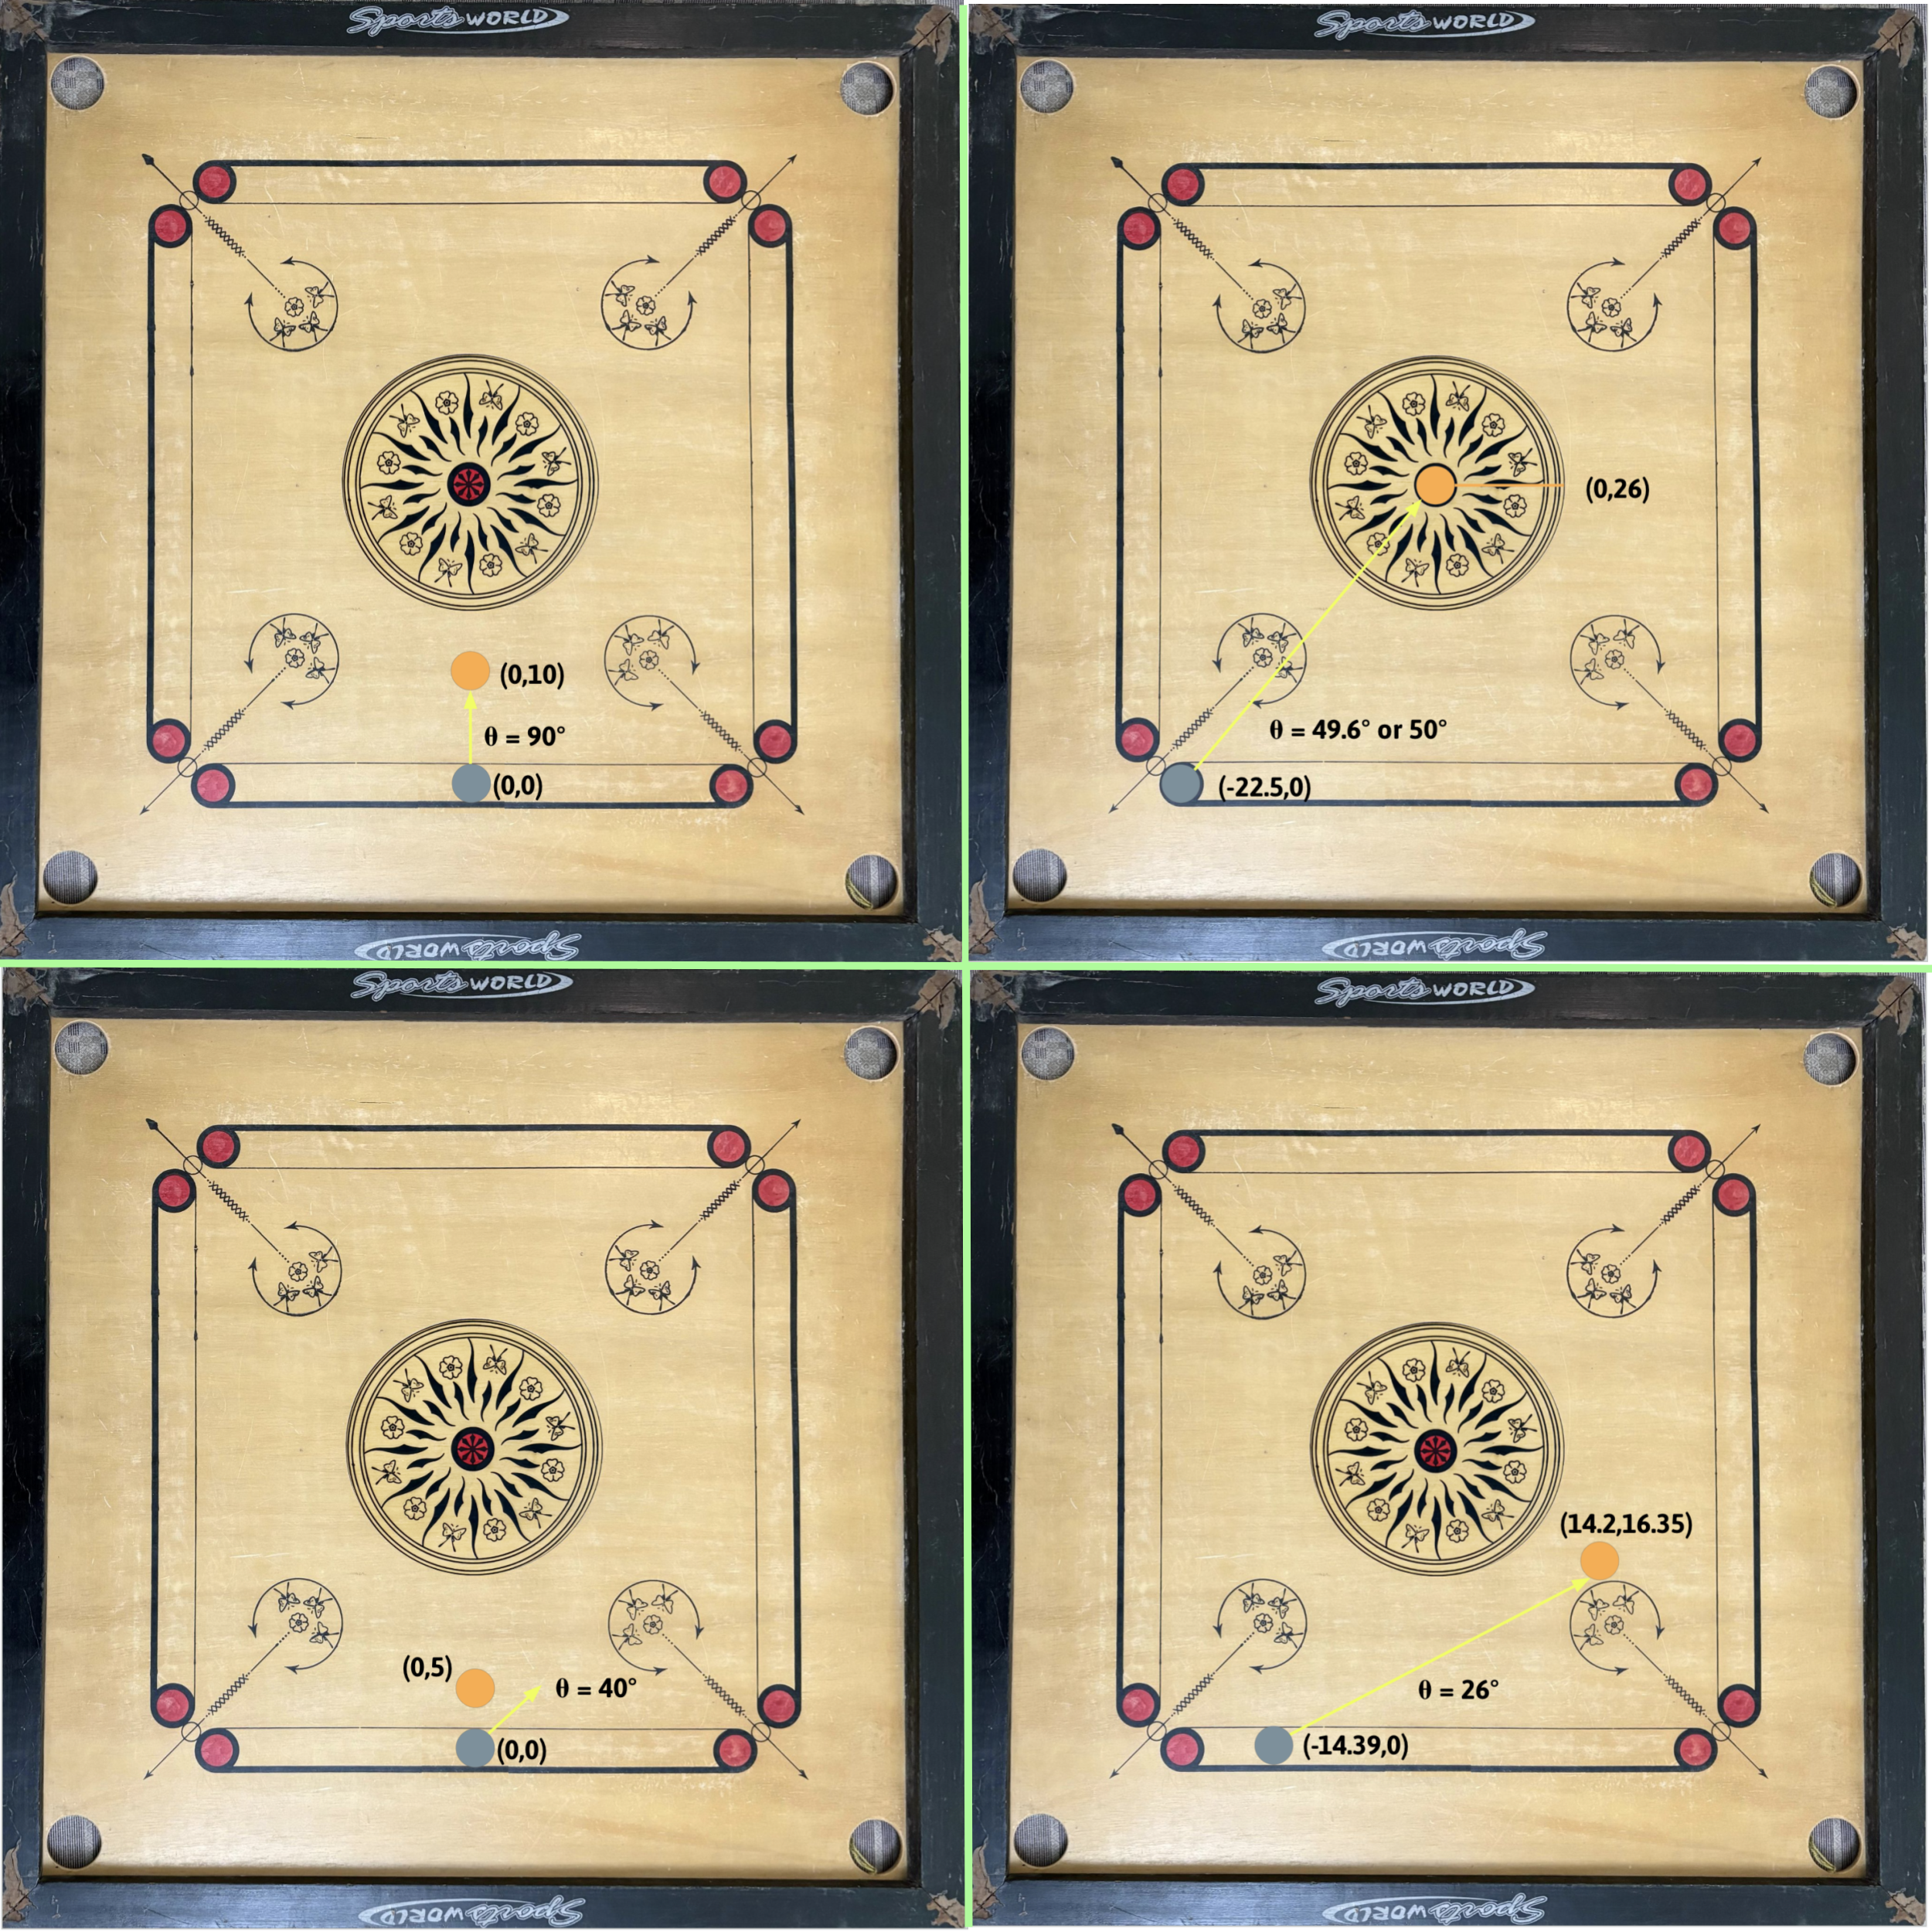
\includegraphics[width=0.5\linewidth]{Method1Examples.png}
    \caption{Diagram Demonstration of Each Row of Table \ref{tab:collision_data}}
    \label{fig:m1diagram}
\end{figure}  


In Figure \ref{fig:m1diagram}, each row of the table is clearly diagramically demonstrated on a carromboard. Row 1, represented by the top left square, shows a simple straight hit upwards, which clearly does not go in the pot and results in a high 34$^{\circ}$ deviation. Row 2 and 3, at the top right, show a hit diagonal from the leftmost striker position to get the centre coin in. At 50$^{\circ}$ initially, the angular deviation is 3.6$^{\circ}$, which based on estimates is not likely to go in, while at 49.6$^{\circ}$, the deviation will be 0.046$^{\circ}$ which can surely go in -- hence highlighting the sensitivity of this function to minute changes in angle. Row 4, the bottom left square, is a shot that misses the coin entirely, and clearly results in a function output of $\pi$, or $180^{\circ}$ as $d>3.5$. Finally, row 5 shows an arbitrary collision that is clearly glancing, where the striker is hit in a way that the coin's motion is at a significant angle to its initial motion, and results in the coin's motion being 1.16$^{\circ}$ off, which means it is possible for it to go into the right pot. 

The function may also be graphed on a 2D plane with a fixed value for all inputs except theta, where the x-axis represents $\theta$ and the y-axis represents $f$. For the fixed values of Row 1, this is shown in Figure  \ref{fig:m1examples}.\footfullcite{desmos_desmos}

\begin{figure}[h]
    \centering
    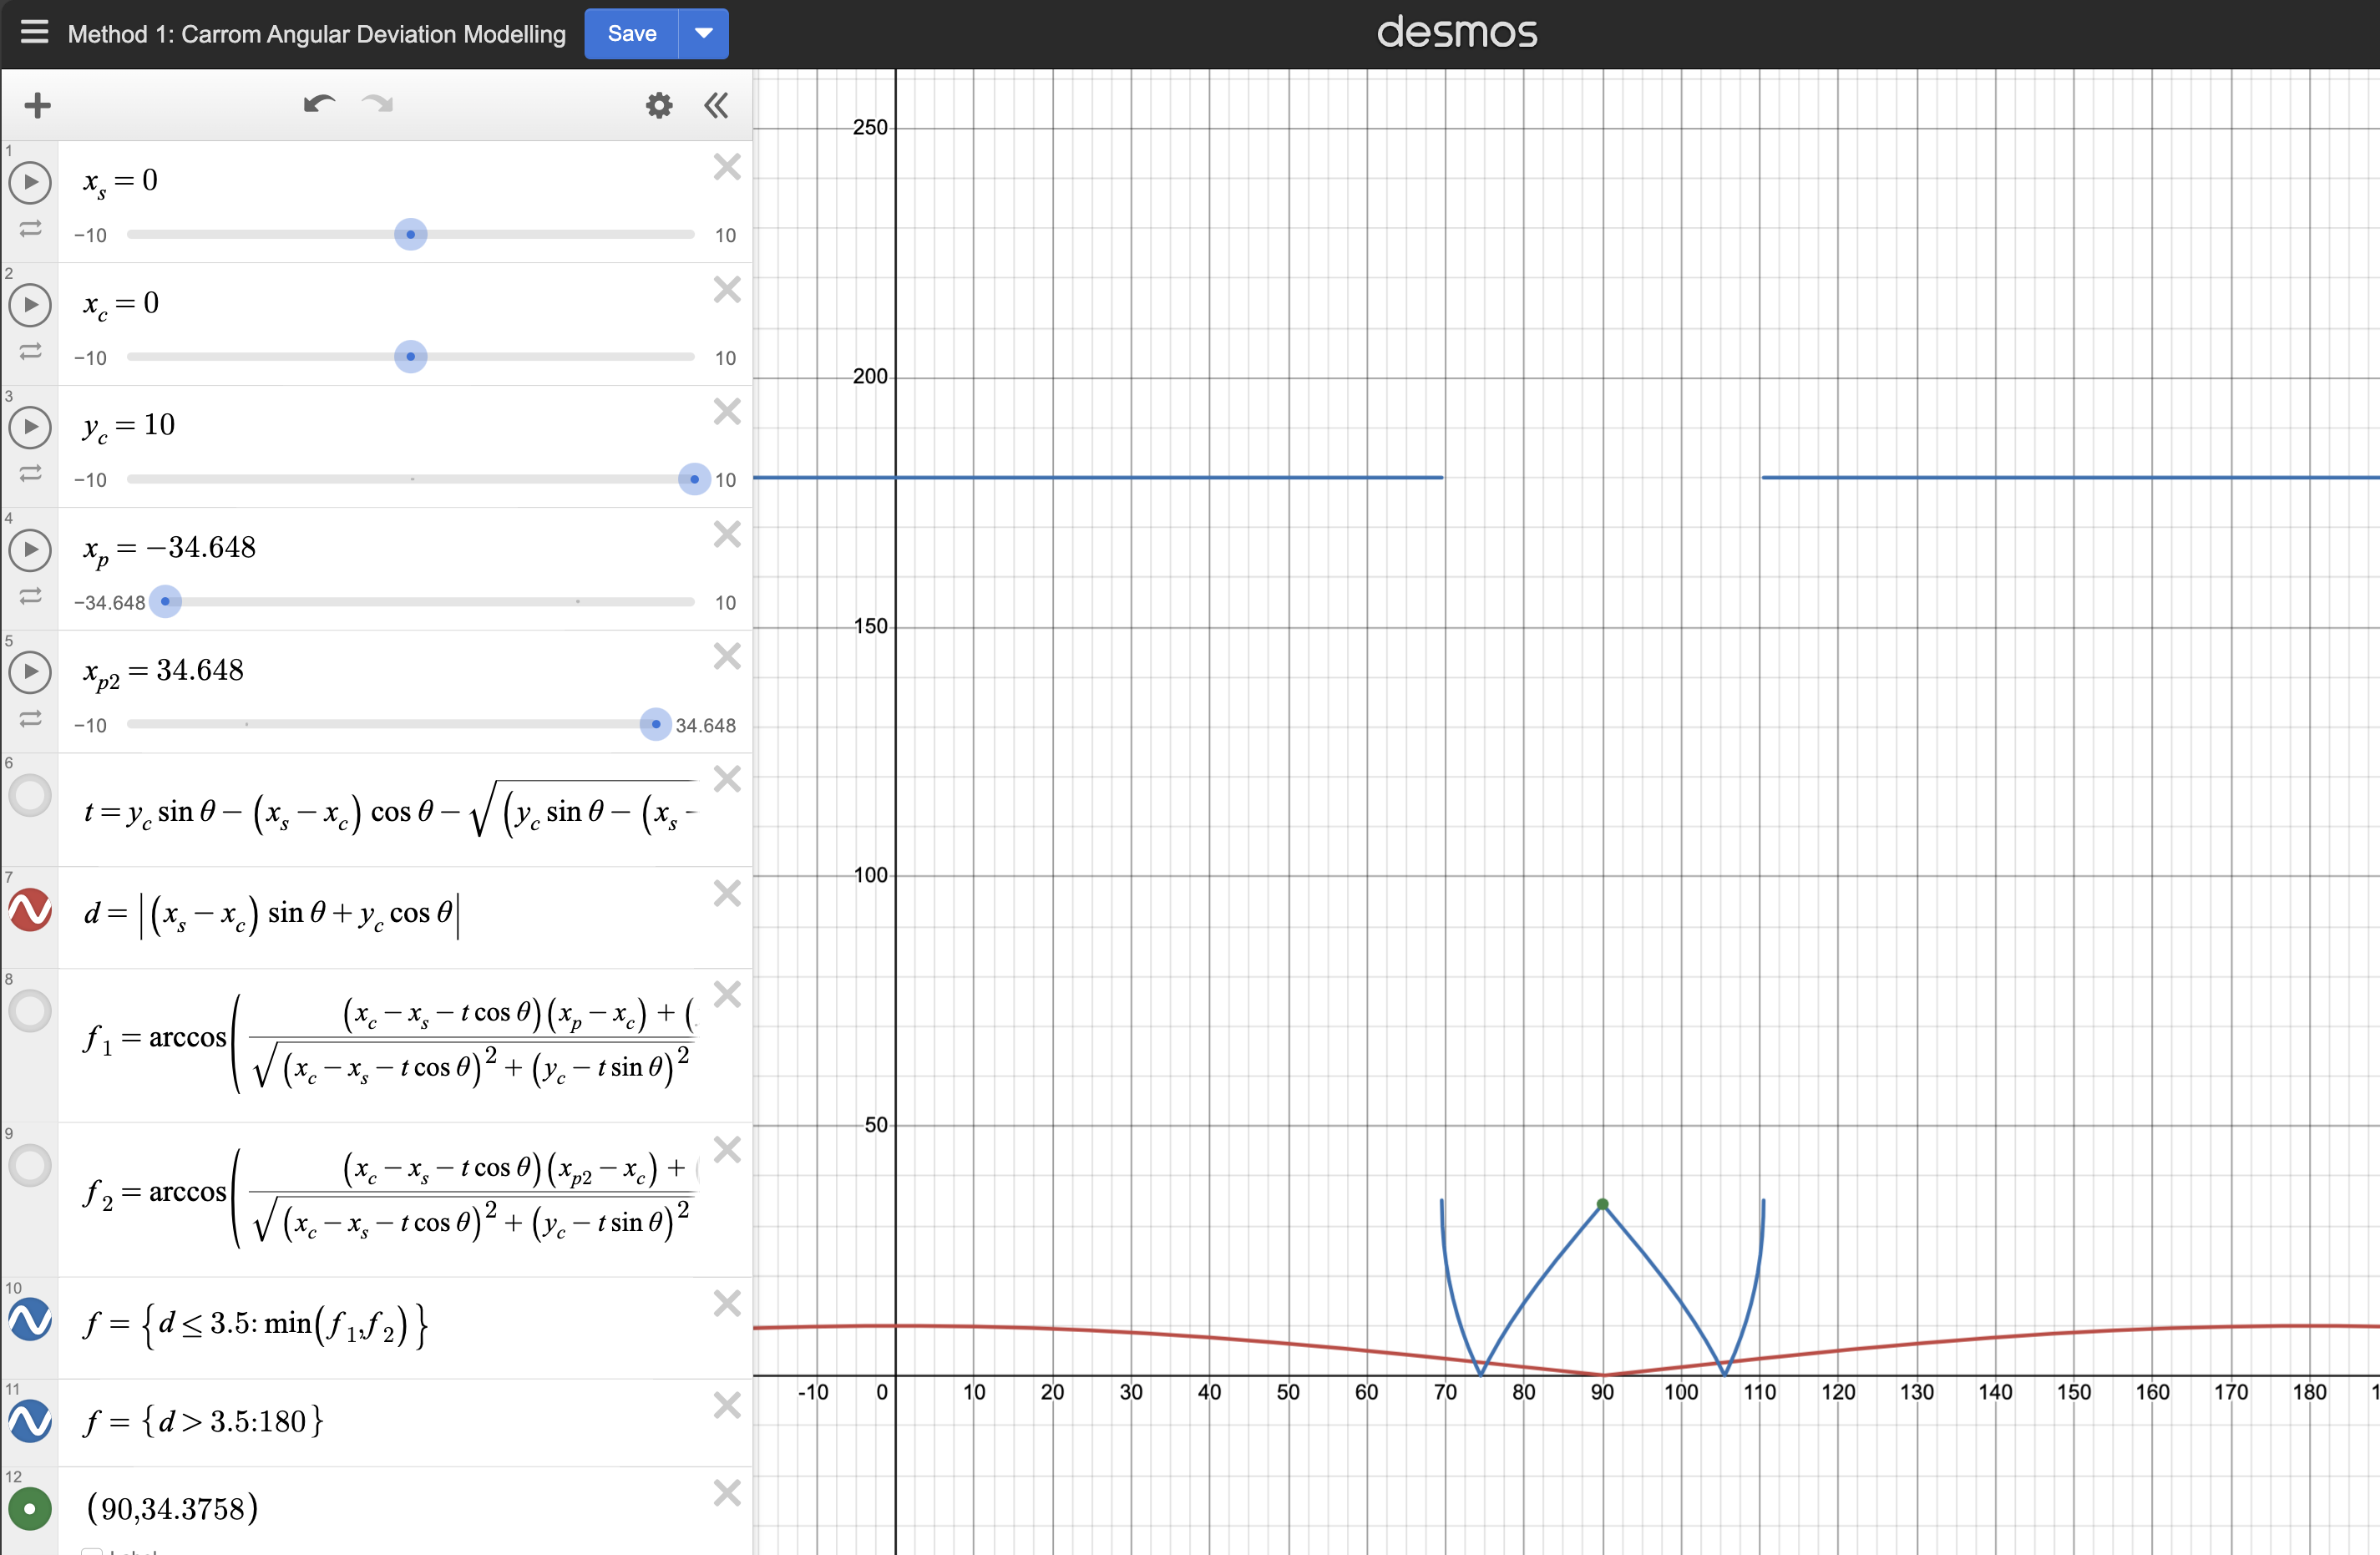
\includegraphics[width=0.5\linewidth]{M1R1Graphed.png}
    \caption{Graphical Representation of Row 1 of Table \ref{tab:collision_data}}
    \label{fig:m1examples}
\end{figure}  


Note that whether it actually goes in for each row with an angular deviation below ~$3^{\circ}$ can depend on factors including velocity, and friction, which are not modelled as per this method. The masses are also not actually equal, so hence it becomes clear that another method must be adopted to accurately model the required conditions for a coin to go into the pot that considers such factors. 

For a smooth, polished carromboard surface with boric acid for smoothening, it may be assumed that the coefficient kinetic friction is between 0.02 to 0.06 -- so let us take an estimate of $\mu_k = 0.04$. 



\section{Method 2: Considering Velocity, Friction, and Masses} 

While Method 1 provides a baseline geometric framework, it fails to account for friction and mass, and hence it is insufficient for practical modeling. We must consider masses, friction, and velocity, as to model the accuracy of a carromboard shot we must look at the distance to the pot after the coin stops (0 if it has entered the pot). 

The first step is to similarly model the collision, but now by considering the initial velocity and friction, as this will tell us velocity of striker upon collision, and hence the direction and velocity of the coin right after collision, and as a result it may be calculated where the coin ends up and if it passes through the pot.

\subsection{Considering Motion Until the Collision}

\subsubsection{Collision Checking Condition}
The collision condition from the previous method still applies, as the initial path of the striker is still the same:
\[
|(x_s - x_c)\sin\theta+y_c\cos\theta| \leq 3.5
\]

However, an extra condition is now required that considers the striker stopping before it even reaches the coin.

The first step of checking the collision can be simply done by first taking the vector from the striker to coin, $\vec{SC} = (x_c-x_s,y_c)$, and the initial direction of striker's movement, $\vec{d}=(\cos\theta, \sin\theta)$.

Let us take the projection $L$ of $\vec{SC}$ onto $\vec{d}$, the direction of motion, to check the distance on the line of travel, through a dot product: $L = \vec{SC} \cdot \vec{d} = (x_c-x_s)\cos\theta+y_c\sin\theta$

This is effectively the distance to the coin along the path of the striker, meaning the striker must travel $L-3.5$ to reach the coin (considering the first collision inequality is true and the coin lies in the striker's path). 

We can now model if the coin will stop before this point with elementary physics. 

Considering the force of friction is $u_kN = u_kmg$, where $N$ is normal force and g is the constant gravitational acceleration of $980$ cms$^{-1}$, we can state through Newton's second Law $F=ma$ that the deceleration of the coin is given by $u_kg$. This is clearly negative in the context of acceleration in direction of motion, hence $a=-u_kg$.

By the kinematics equation $v^2=v_0^2 + 2as$, where $s$ is the distance the striker will reach at a certain velocity $v$, and $v_0 = v_s$ (initial velocity of striker), let us find $s$ if $v=0$:

\[
0=v_s^2 + 2(-u_kg)s \longrightarrow 2u_kgs=v_s^2 \longrightarrow s=\frac{v_s^2}{2u_kg}
\]

Substituting the estimated $u_k = 0.04$ and $g=980$ cms$^{-1}$, we have $s=\frac{v_s^2}{78.4}$. This is the stopping distance, and it must be greater than the required travel distance of $L-3.5$ derived earlier. Hence, for the function to be calculated, the following inequality must hold true:
\[
\frac{v_s^2}{78.4} \geq L-3.5 \longrightarrow v_s^2 \geq 78.4[(x_c-x_s)\cos\theta+y_c\sin\theta - 3.5]
\]

\subsubsection{Position and Velocity of Striker Upon Collision} 

The position can still be calculated in the exact same way as Method 1, as the position upon collision is not impacted by velocity and friction, and the condition checking inequalities will ensure it occurs. However, it must be noted that $t$ in this scenario cannot represent time in any manner and is simply a scalar quantity to represent the set of points along the line -- a certain value of $t$ can hence be considered as a scalar distance, not a time. Let us hence replace $t$ with $s$ in this scenario, where $s$ represents distance from initial striker position to collision position in centimeters.

The position $P$ is hence:

\[
P = S+s\vec{d} = (x_s,0)+s(\cos\theta,\sin\theta) =\left( x_s + s \cos \theta,\ s \sin \theta \right)
\]

Where $s$ is given by:

\[
s = -\left[\cos \theta (x_s - x_c) - \sin \theta y_c\right] 
- 
\sqrt{
\left[\cos \theta (x_s - x_c) - \sin \theta y_c\right]^2 
- 
\left[(x_s - x_c)^2 + y_c^2 - 12.25\right]
}
\]

We already know the distance $s$, which may now be substituted in kinematics equations to find the velocity $v_{a}$ of the striker upon collision.

\[
v_a^2 = v_s^2+2as=v_s^2 - 2u_kgs
\]

Thus, the magnitude of this velocity, substituting $u_k = 0.04$ and $g=980$ is:

\[
v_a = \sqrt{v_s^2 - 78.4s}
\]

The vector of this initial velocity of the striker, since the direction is given by $\vec{d} = (\cos\theta,\sin\theta)$ is:

\[
\vec{v_a} = \sqrt{v_s^2 - 78.4s} \cdot (\cos\theta,\sin\theta)
\]

\subsection{Calculating the Impact of the Collision on Velocities}
Now, based on the collision, the resulting vector of the coin's motion can be calculated.\footfullcite{tatum_2017_54} The known values, in terms of the function inputs, are:
\begin{outline}
    \1 Striker: mass = $m_s = 5$ g $= 0.005$ kg, velocity = $v_a$, position = $\left( x_s + s \cos \theta,\ s \sin \theta \right)$
    \1 Coin: mass = $m_c = 7$ g $= 0.007$ kg, velocity = 0, position = $(x_c,y_c)$
    \1 e = 0.9 (coefficient of restitution)
    \1 Direction of Impact: Striker centre  to coin centre (find $\hat{n}$)
    \1 2D components:
        \2 The collision along the line $\hat{n}$ (normal component)
        \2 The tangential (perpendicular) component remains unchanged
\end{outline}

Let us first find the value of $\hat{n}$. Taking the position of striker at collision as $P$ and position of coin as $C$ this is found by:

\[
\hat{n} = \frac{\vec{C}-\vec{P}}{\|\vec{C}-\vec{P}\|} = \frac{(x_c, y_c)-( x_s + s \cos \theta,\ s \sin \theta)}{\|(x_c, y_c)-( x_s + s \cos \theta,\ s \sin \theta)\|}
\]
Simplifying:
\[
\hat{n} = \frac{(x_c - x_s - s \cos \theta, y_c - s\sin\theta)}{\|(x_c - x_s - s \cos \theta, y_c - s\sin\theta)\|} = \frac{(x_c - x_s - s \cos \theta, y_c - s\sin\theta)}{\sqrt{(x_c - x_s - s \cos \theta)^2 + (y_c - s\sin\theta)^2}}
\]
Keeping this as our value of $\hat{n}$, let us find the velocity along $\hat{n}$, the normal component, which is the only direction in which the collision force will ideally act.

The magnitude of the striker's initial velocity along the normal component is:
\[
v_{an} = \vec{v_a} \cdot \hat{n} = \sqrt{\frac{v_s^2 - 78.4s}{(x_c - x_s - s \cos \theta)^2 + (y_c - s\sin\theta)^2}} \left(x_c\cos\theta - x_s\cos\theta - s \cos^2 \theta + y_c\sin\theta - s\sin^2\theta\right)\]
The coin has 0 velocity, so let us take $v_{bn} = 0$ (the coin's velocity along the normal component).

Let us now consider the coefficient of restitution, $e$, which measures elasticity of a collision and models how much energy is lost. A reasonable estimate for $e$ in a carromboard striker and coin collision is $e = 0.90$. $e$ is defined by the formula:

\[
e = \frac{v_{bn}' - v_{an}'}{v_{an} - v_{bn}} = \frac{v_{bn}' - v_{an}'}{v_{an}} \quad \text{(since } v_{bn} = 0 \text{)}
\]

$v_{bn}'$ and $v_{an}'$ represent the coin's velocity after, and the striker's velocity after, respectively, so by the law of conservation of momentum($m_s v_{an} + m_cv_{bn} = m_sv_{an}' + m_c v_{bn}'$):
\[
\text{Substituting $v_{bn} = 0$, $m_s = 0.005$ kg, and $m_c = 0.007$ kg: }0.005v_{an} = 0.005v_{an}' + 0.007v_{bn}'
\]
\[
\text{We also know: } e = \frac{v_{bn}' - v_{an}'}{v_{an}} \rightarrow 0.9 = \frac{v_{bn}' - v_{an}'}{v_{an}}
\]
Using simultaneous equations to find $v_{bn}'$ in terms of $v_{an}$:
\[
\begin{cases}
    0.9v_{an} = v_{bn}' - v_{an}' \\
    0.005v_{an} = 0.005v_{an}' + 0.007v_{bn}'
\end{cases}
\rightarrow
\begin{cases}
    0.9v_{an} + v_{an}' = v_{bn}'  \\
    v_{an} - v_{an}' =  1.4v_{bn}'
\end{cases}
\]
\[
\text{Adding both, }   1.9v_{an} = 2.4v_{bn}', \text{hence } v_{bn}' = \frac{19v_{an}}{24} = \frac{19(\vec{v_a} \cdot \hat{n})}{24}
\]
\[
= \frac{19}{24} \sqrt{\frac{v_s^2 - 78.4s}{(x_c - x_s - s \cos \theta)^2 + (y_c - s\sin\theta)^2}} \left(x_c\cos\theta - x_s\cos\theta - s \cos^2 \theta + y_c\sin\theta - s\sin^2\theta\right)
\]
Let us call the speed of the coin $v_c = v_{bn}'$ and the velocity vector $\vec{v_c}$.

To obtain this velocity vector, $v_c$ must be multiplied by $\hat{n}$:
\[
\vec{v_c} = \frac{19}{24} \sqrt{\frac{v_s^2 - 78.4s}{(x_c - x_s - s \cos \theta)^2 + (y_c - s\sin\theta)^2}} \left(x_c\cos\theta - x_s\cos\theta - s \cos^2 \theta + y_c\sin\theta - s\sin^2\theta\right) \cdot \hat{n}
\]
\[
= \frac{19\sqrt{v_s^2 - 78.4s} \left(x_c\cos\theta - x_s\cos\theta - s \cos^2 \theta + y_c\sin\theta - s\sin^2\theta\right)}{24((x_c - x_s - s \cos \theta)^2 + (y_c - s\sin\theta)^2)}  \cdot (x_c - x_s - s \cos \theta, y_c - s\sin\theta)
\]

Now the velocity vector $\vec{v_c}$ of the coin after collision is known considering friction, masses, and restitution.

\subsection{Calculating the Stopping Point And Distance to the Pot}

Note that the coin's direction and initial path of movement is still going to be the same in this model as in Method 1, but the difference is the involvement of velocity and deceleration which lets us calculate the stopping point.

If the stopping point is before the pot, the function should return the distance of this point to the pot. If it hits a wall, as this function does not consider wall bounces, the distance of the point where it hits to the pot will be taken. If it passes past or into the pot, certain parameters will help us decide whether or not to return a distance of 0.

\subsubsection{Calculating the Stopping Point Of the Coin}

The stopping distance $d_s$ can be given by the same formula as earlier, $d_s = \frac{v_c^2}{2u_kg}$, by just replacing initial velocity, as the deceleration is the same (given by $a = -u_kg$). This is the distance the coin will move in the same direction as $\hat{n}$. We can multiply this direction by the unit vector to get the displacement vector from $(x_c,y_c)$ to the stopping point, and replace $u_k = 0.04$ and $g=980$:
\[
\small
\vec{d_s} = \frac{v_c^2(x_c - x_s - s \cos \theta, y_c - s\sin\theta)}{78.4\sqrt{(x_c - x_s - s \cos \theta)^2 + (y_c - s\sin\theta)^2}}
\]

Finally, adding the displacement vector to the coin's initial position $(x_c,y_c)$ provides the stopping point $P_s$:
\begin{align*}
\small
P_s = \Bigg(
    &x_c + \frac{v_c^2(x_c - x_s - s \cos \theta)}
    {78.4 \sqrt{(x_c - x_s - s \cos \theta)^2 + (y_c - s \sin \theta)^2}}, 
    &y_c + \frac{v_c^2(y_c - s \sin \theta)}
    {78.4 \sqrt{(x_c - x_s - s \cos \theta)^2 + (y_c - s \sin \theta)^2}}
\Bigg)
\end{align*}

With $s$ given by:

\[
\small
s = -\left[\cos \theta (x_s - x_c) - \sin \theta y_c\right] 
- 
\sqrt{
\left[\cos \theta (x_s - x_c) - \sin \theta y_c\right]^2 
- 
\left[(x_s - x_c)^2 + y_c^2 - 12.25\right]
}
\]

\subsubsection{Considering the Walls and Pot}

Through the measurements taken earlier, we can estimate the walls to be at y = 63.05, x = 37.05, and x = -37.05. 

Let us then formulate an expression for the distance that must be travelled along the direction $\hat{n}$ in which the coin travels, for the coin to reach any of the walls, considering radius of 1.5 cm.
\[
\text{Right Wall: } \hat{n}_x > 0 \rightarrow d_r = \frac{35.55 - x_c}{\hat{n}_x}, \text{ Left Wall: } \hat{n}_x < 0 \rightarrow d_l = \frac{-35.55 - x_c}{\hat{n}_x}
\]
\[
\text{Upper Wall: }\hat{n}_y > 0 \rightarrow d_u = \frac{61.55 - y_c}{\hat{n}_y}
\]

To make this more elegant, let us first assume that $\hat{n}_y > 0$ as in standard carrom play, a striker shot upwards will aim for potting the coin in one of the top pots, and hence will not be at such an unusual angle that the coin moves backwards. Secondly, the constraint for the left and right wall can be modelled neatly with a signum function -- which returns 1 for positive numbers, 0 for 0, and -1 for negative numbers. Let us write it as:
\[
d_x = \frac{x_{wall} - x_c}{\hat{n}_x}
= \frac{35.55 \cdot \text{sgn}(\hat{n}_x) - x_c}{\hat{n}_x}
\]

However, this will later lead to issues in differentiation, and dividing by 0 becomes an issue, so let us tweak this by adding a small epsilon in the denominator ($\varepsilon = 10^{-6}$) and replacing signum with hyperbolic tan, as in $\tanh(kx)$, large values of $k$ make the function approximate $\text{sgn}(x)$. 

\[
d_x = \frac{35.55 \cdot \tanh(100\hat{n}_x) - x_c}{\hat{n}_x + \varepsilon}
\]

Now, let us take the minimum of these distances as what the striker must travel to hit a wall, such that $d_{wall} = \min(d_x,d_u)$. Hence the final position that will be taken based on these calculations is:
\[
P_{stop} =
\begin{cases}
P_s & \text{if } d_s < d_{\text{wall}} \\
(x_c, y_c) + \hat{n} \cdot d_{wall} & \text{otherwise}
\end{cases}
\]
\[
\text{Replacing values: } P_{stop} =
\begin{cases}
(x_c,y_c) + \frac{v_c^2 \cdot \hat{n}}{78.4} & \text{if } d_s < d_{\text{wall}} \\
(x_c, y_c) + \hat{n} \cdot \min(\frac{35.55 \tanh(100\hat{n}_x) - x_c}{\hat{n}_x + 10^{-6}},\frac{61.55 - y_c}{\hat{n}_y}) & \text{otherwise}
\end{cases}
\]

Now, considering if a coin will pass through the pot, as the pot has a radius of 2.4 cm, let us put a distance of 0 if the centre of the coin passes through any part of the circular pot, else the distance returned will be that of the stopping point.
\[
\text{distance} =
\begin{cases}
0, & \text{if } 
\begin{cases}
0 \leq s_1 \leq d_{s} \text{ and } d_1 \leq 2.4, \quad \text{or} \\
0 \leq s_2 \leq d_{s} \text{ and } d_2 \leq 2.4
\end{cases} \\
d_{\text{stop}}, & \text{otherwise}
\end{cases}
\]

In this, $s_1$ and $s_2$ represent the required distance the coin travels along the line of motion for it to reach pots 1 and 2, respectively, and $d_s$ is the stopping distance already found. $d_1$ and $d_2$ each represent the distance of the centre of the respective pot to the closest point on the line of motion. Finally, $d_{\text{stop}}$ is the distance of $P_{stop}$ to the closest pot. Now let us find each of these values and finally state the function in terms of the inputs.

To find the values of $s_1$ and $s_2$, let us take the x of the pots as $x_{p_i}$ and $y_{p_i}$ for now, for $i = 1,2$. The required distance $s_i$ is the dot product of the vector from coin to pot with the line of motion's direction vector:
\[
s_i = (x_{p_i} - x_c,\ y_{p_i} - y_c) \cdot \hat{n} = (x_{p_i} - x_c)n_x + (y_{p_i} - y_c)n_y
\]

To find the minimum distance between centre of pot and line of motion, we take the vector of the coin travelling a distance of $s_i$ along $\hat{n}$ and take the difference between this vector and the one directly from coin to pot. This would result in a vector from the closest the coin goes to the pot, to the centre of the pot, and the magnitude of this must be less than or equal to the radius (2.4 cm) of the pot -- hence this magnitude is our $d_i$.

\[
d_i = \left\| (x_{p_i} - x_c,\ y_{p_i} - y_c) - s_i \hat{n} \right\| = 
\sqrt{(x_{p_i} - x_c - s_i n_x)^2 + (y_{p_i} - y_c - s_i n_y)^2}
\]

Now, the value of $d_{\text{stop}}$ is essentially the minimum of the distance of $P_{stop}$ to each pot, hence using the point distance formula:

\[
d_{\text{stop}} = \min\left(\|P_{stop} - (-34.648, 60.648)\|,\|P_{stop} - (34.648, 60.648)\|\right)
\]
Considering the piecewise $P_{stop}$, and taking $\pm34.648$ as the x-coordinate to reduce repetitiveness:
\[
=
\begin{cases}
\min\left(\|P_{s} - (\pm34.648, 60.648)\|\right) & \text{if } d_s < d_{wall} \\
\min\left(\|(x_c,y_c) + \hat{n} \cdot d_{wall} - (\pm34.648, 60.648)\|\right) & \text{otherwise}
\end{cases}
\]
Remembering the distance formula is $\sqrt{(x_2 - x_1)^2 + (y_2 - y_1)^2}$:

\[
=
\begin{cases}
\min\left(
\sqrt{(\pm34.648 - x_c - \frac{v_c^2 \hat{n}_x}{78.4})^2 + (60.648 - y_c - \frac{v_c^2 \hat{n}_y}{78.4})^2}
\right) & \text{if } d_s < d_{wall} \\
\min\left(\sqrt{(\pm34.648 - x_c - d_{wall} \cdot \hat{n}_x)^2 + (60.648 - y_c - d_{wall}\cdot\hat{n}_y)^2}\right) & \text{otherwise}
\end{cases}
\]

Let us write $d_s$ as $\frac{v_c^2}{78.4}$, and obtain our final distance expression, with the binary variable $p$ to represent the coin being potted. 
\[
\normalsize
\begin{cases}
0 & \text{if } 
p\\
    \min\left(
    \sqrt{(\pm34.648 - x_c - \frac{v_c^2 \hat{n}_x}{78.4})^2 + (60.648 - y_c - \frac{v_c^2 \hat{n}_y}{78.4})^2}
    \right) & \text{otherwise if } \frac{v_c^2}{78.4} < d_{wall} \\
\min\left(\sqrt{(\pm34.648 - x_c - d_{wall} \cdot \hat{n}_x)^2 + (60.648 - y_c - d_{wall}\cdot\hat{n}_y)^2}\right) & \text{otherwise}
\end{cases}
\]

Where, with the constants $y_p = 60.648$, $x_{p1} = -34.648$ and $x_{p2} = 34.648$ to reduce spacing, $p =$:
\[
\footnotesize
\Bigg( \Bigg(
0 \leq (x_{p1} - x_c)\hat{n}_x + (y_{p} - y_c)\hat{n}_y \leq \frac{v_c^2}{78.4} \Bigg)\text{ and }
\]
\[
\footnotesize
\Bigg(\\\sqrt{(x_{p1} - x_c - ((x_{p1} - x_c)\hat{n}_x + (y_{p} - y_c)\hat{n}_y) \hat{n}_x)^2 + (y_{p} - y_c - ((x_{p1} - x_c)\hat{n}_x + (y_{p} - y_c)\hat{n}_y) \hat{n}_y)^2}  \leq 2.4 \Bigg) \Bigg)
\]
\[
\footnotesize
 \lor \Bigg( \Bigg(
0 \leq (x_{p2} - x_c)\hat{n}_x + (y_{p} - y_c)\hat{n}_y \leq \frac{v_c^2}{78.4} \Bigg) \land
\]
\[
\footnotesize
\Bigg( \sqrt{(x_{p2} - x_c - ((x_{p2} - x_c)\hat{n}_x + (y_{p} - y_c)\hat{n}_y) \hat{n}_x)^2 + (y_{p} - y_c - ((x_{p2} - x_c)\hat{n}_x + (y_{p} - y_c)\hat{n}_y) \hat{n}_y)^2}  \leq 2.4 \Bigg) \Bigg)
\]


And $d_{wall}$, $(\hat{n}_x,\hat{n}_y)$, $v_c$, and $s$ each are equal to:

\[
\small
d_{wall} = \min(\frac{35.55 \tanh(100\hat{n}_x) - x_c}{\hat{n}_x + 10^{-6}},\frac{61.55 - y_c}{\hat{n}_y})
\]

\[
\hat{n} = (\hat{n}_x,\hat{n}_y) = \frac{(x_c - x_s - s \cos \theta, y_c - s\sin\theta)}{\sqrt{(x_c - x_s - s \cos \theta)^2 + (y_c - s\sin\theta)^2}}
\]
\[
v_c = \frac{19}{24} \sqrt{\frac{v_s^2 - 78.4s}{(x_c - x_s - s \cos \theta)^2 + (y_c - s\sin\theta)^2}} \left(x_c\cos\theta - x_s\cos\theta - s \cos^2 \theta + y_c\sin\theta - s\sin^2\theta\right)
\]
\[
\small
s = -\left[\cos \theta (x_s - x_c) - \sin \theta y_c\right] 
- 
\sqrt{
\left[\cos \theta (x_s - x_c) - \sin \theta y_c\right]^2 
- 
\left[(x_s - x_c)^2 + y_c^2 - 12.25\right]
}
\]
\[
\text{Domain: } v_s^2 \geq 78.4[(x_c-x_s)\cos\theta+y_c\sin\theta - 3.5]
\]

\section{Optimizing Both Methods And Analysing}

\subsection{Optimizing Method 2 Numerically To Find Easiest Coin Placements}
Method 2 accurately models the distance to the pot when inputs regarding the details are provided. However, solely focusing on the binary function p, which states whether a coin enters a pot, allows us to calculate what coin positions are optimum through a brute force numerical (programmatic) method. 

By implementing the derived binary function $p$ programatically in Python, a score function was developed with parameters $(x_c,y_c,v_s)$, to loop through $x_s$ values from -22.5 to 22.5 with a step-size of 0.25. For each $x_s$, it loops through $\theta$ values from $0^{\circ}$ to $180^{\circ}$ with a step size of $0.25^{\circ}$. In each of these specific $\theta$ and $x_s$ values, there is initially a collision check for if the striker collides with the coin given $x_s,\theta,x_c,y_c,v_s$, and if this passes, then only if $p$ returns true, the function adds 1 to the 'score' of this point $(x_c,y_c)$. By looping through all possible $x_s$ and $\theta$ for the point, this $score$ function provides a value determining easiness of potting the coin at the given position, given a striker velocity $v_s$. A value of 0 means the velocity is too low to pot this coin no matter the placement or angle, while values in the thousands mean that this coin can be potted fairly easily in multiple ways without any wall bounces required. Based on this, the $allScores$ function was made which calculated the scores for each point ($x_c,y_c$) with a step size of 0.1 for each coordinate, given a set velocity $v_s$, and returned a 2-dimensional array of these scores for each point. This 2D array was then be converted into a heatmap via Matplotlib, accurately showing the ease of potting a coin at each point in the domain of ($x_c,y_c$) as shown in Figure \ref{fig:heatmapboard180} for $v_s = 180$ cms$^{-1}$.

\begin{figure}[H]
    \centering
    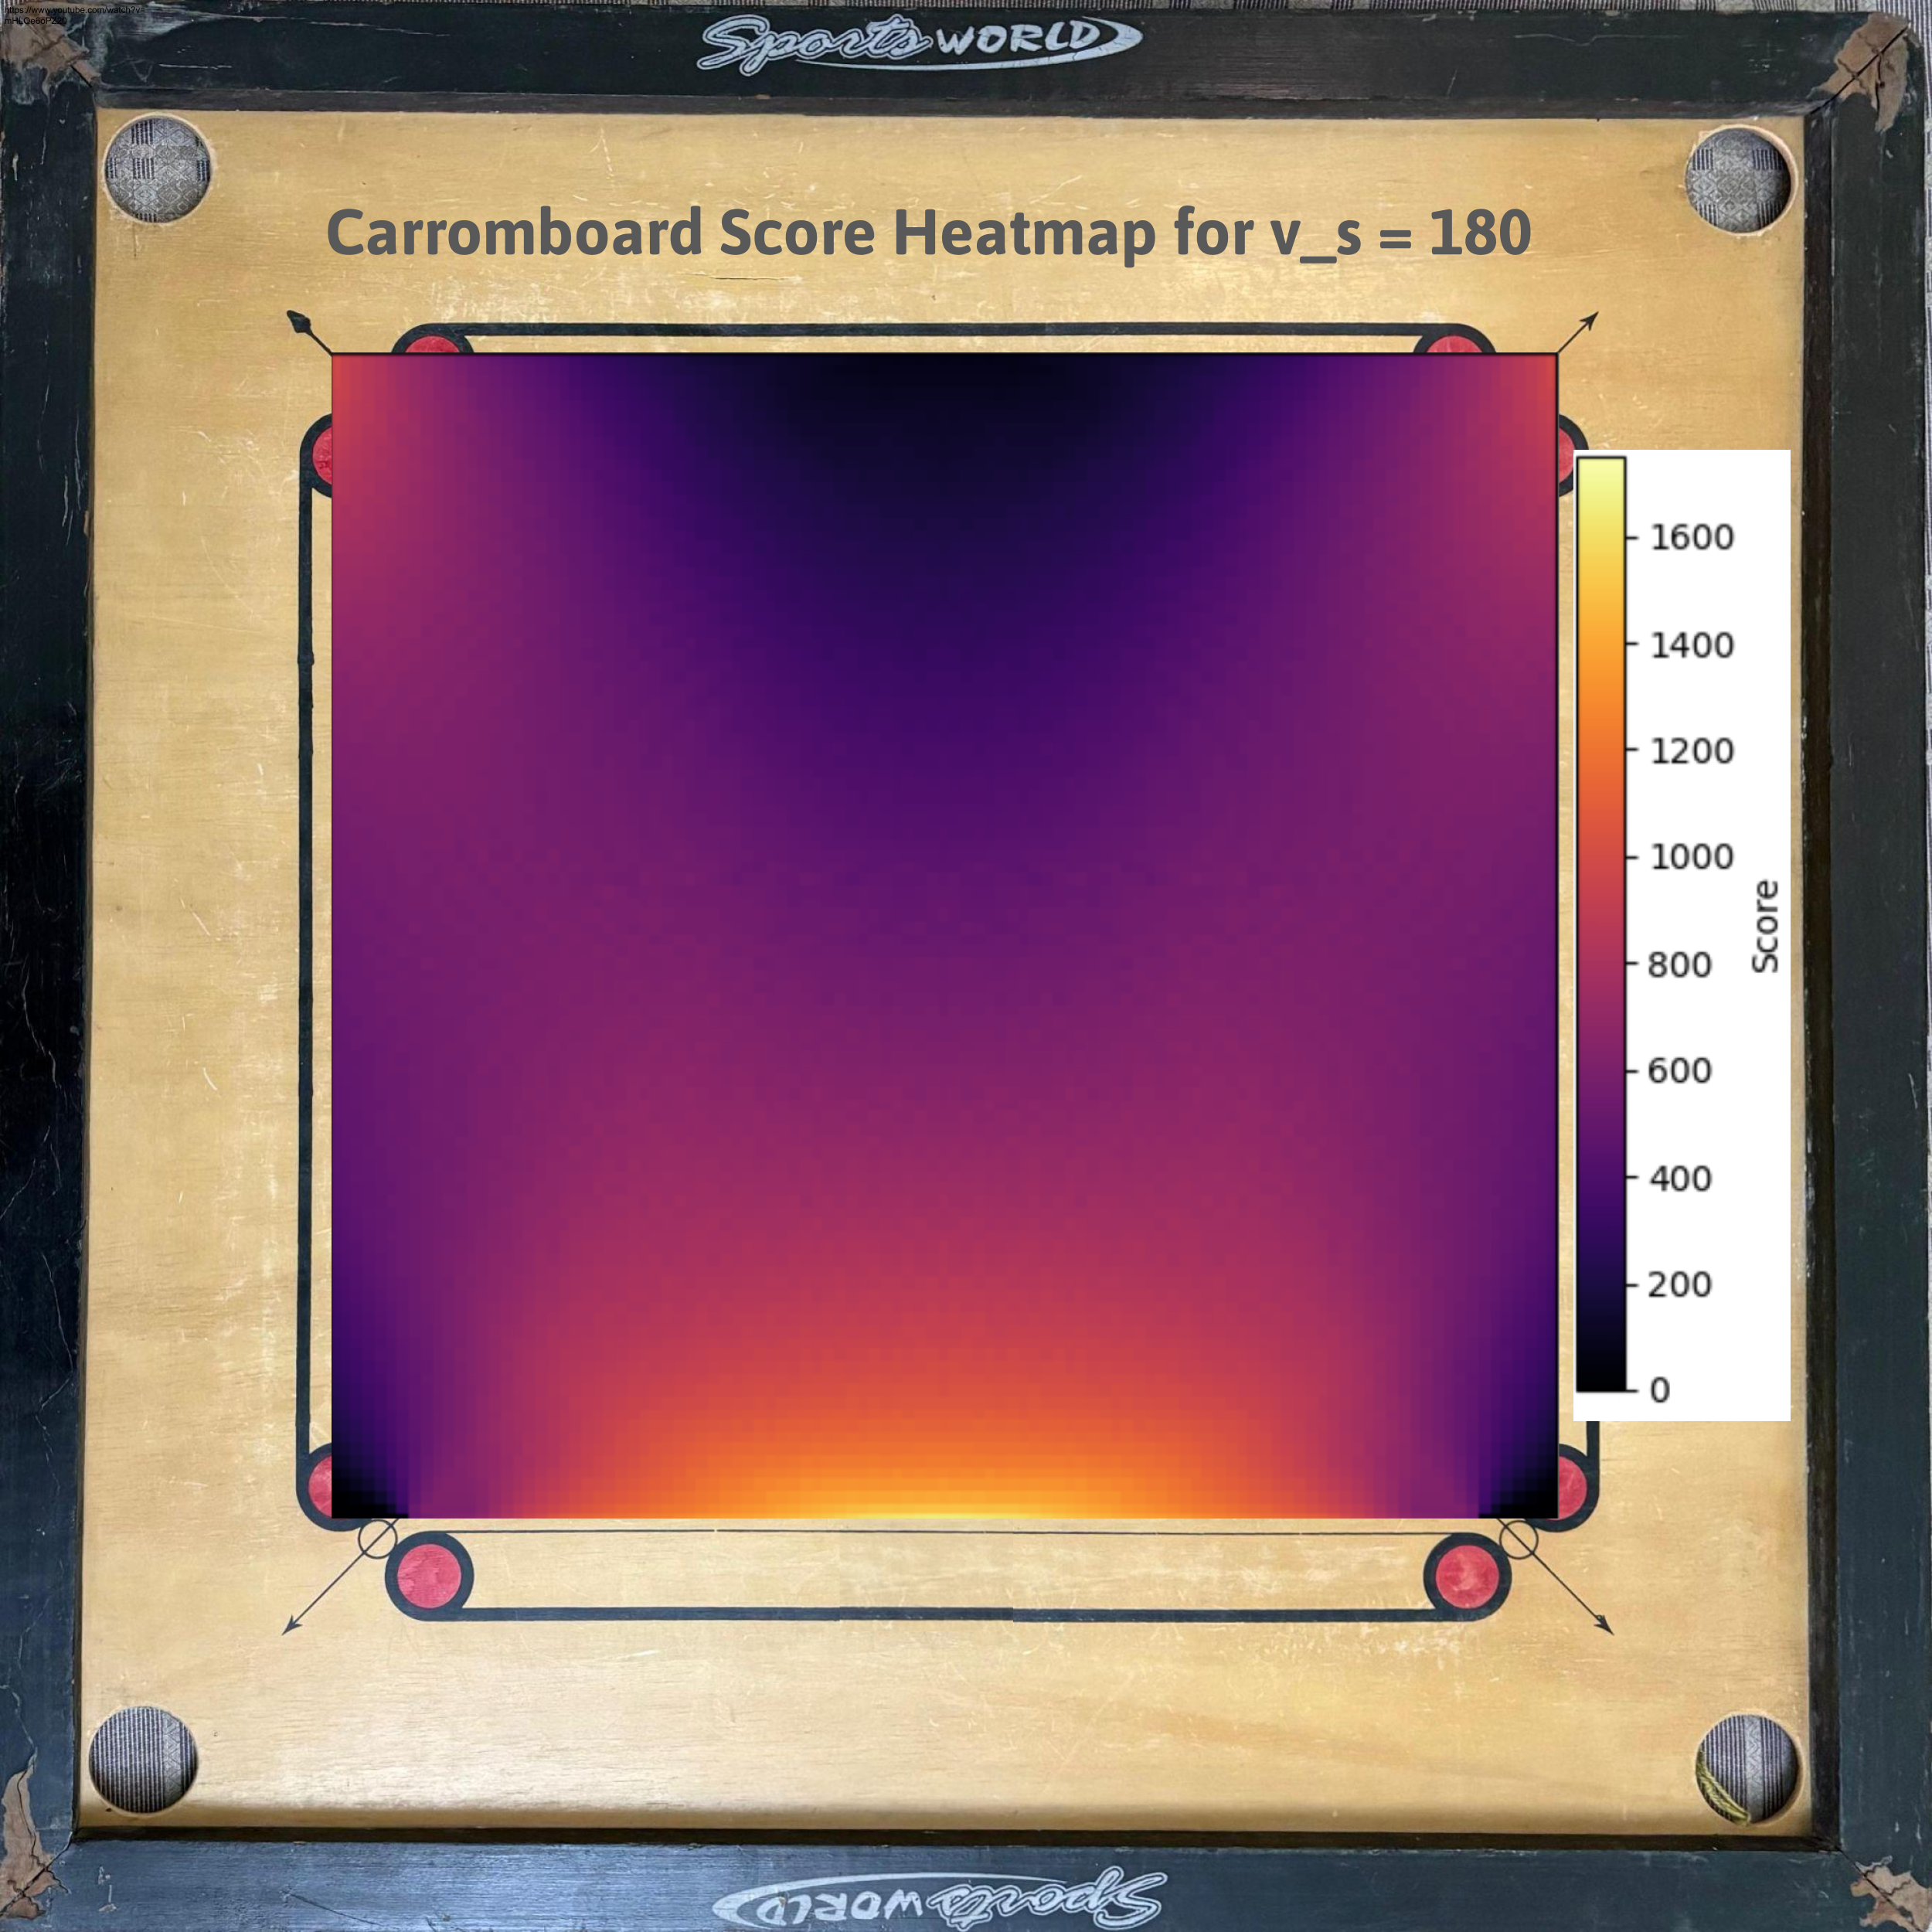
\includegraphics[width=0.5\linewidth]{CarromBoardHeat180.png}
    \caption{Carromboard Score Heatmap of $v_s = 180$ Upon Carromboard}
    \label{fig:heatmapboard180}
\end{figure}

Similarly, such figures were generated for various initial striker velocities, resulting in various observations regarding optimization -- as in the game of carrom, such observations along with a player's own comfortable striker velocity allow players to optimally choose coins to pot which are easier. 


\subsection{Numerically Optimising Method 1 To Find Optimum Striker Shots}

To mathematically analyse Method 1, we can find the optimum striker placement ($x_s$) and angle ($\theta$) for fixed values of ($x_c,y_c$). Through a core concept in multivariable calculus, Hessian matrices, local maxima and minima in a multivariable function can be found.

\subsubsection{Assumptions and Constraints}

The first step is to understand the situation: for any given coin, the optimal shot has $x_s$ and $\theta$ such that the coin can be potted directly (i.e., the function $g(x)$ in Method 1 returns an angular deviation of 0.) For the purposes of this optimization, let us focus on only the right pot: $(x_p,y_p) = (34.648,60.648)$, essentially meaning we are optimising the function $f_2$ from Method 1 with constant $(x_c,y_c)$, where the domain to ensure that a collision occurs is $|(x_s - x_c)\sin\theta+y_c\cos\theta| \leq 3.5$.

\small
\[f_2(\theta,x_s) = \arccos\left(\frac{(x_c-x_s-t\cos\theta)(34.648 - x_c)+(y_c-t\sin\theta)(60.648 - y_c)}{\sqrt{
(x_c-x_s-t\cos\theta)^2 + (y_c-t\sin\theta)^2
}\cdot \sqrt{
(34.648 - x_c)^2 + (60.648 - y_c)^2
}}\right) \]

Where:
\[
t = -\left[\cos \theta (x_s - x_c) - \sin \theta y_c\right] 
- 
\sqrt{
\left[\cos \theta (x_s - x_c) - \sin \theta y_c\right]^2 
- 
\left[(x_s - x_c)^2 + y_c^2 - 12.25\right]
}
\]

\normalsize
Clearly, analytically differentiating $f_2$ for 2 variables with such constraints would require many nested square roots and trigonometric functions, leading to unmanageable formulaic complexity. Hence, numerical partial differentiation and Hessian matrices must be used.

\subsubsection{Hessian Matrices and the Second Derivative Test}
For a function $f(x_s, \theta)$ of two variables, critical points occur where both first-order partial derivatives vanish\footfullcite{hessian}:
\[
\frac{\partial f_2}{\partial x_s} = 0 \quad \text{and} \quad \frac{\partial f_2}{\partial \theta} = 0
\]

To classify these critical points, we use the Hessian matrix, which contains all second-order partial derivatives:
\[
H = \begin{bmatrix}
\frac{\partial^2 f_2}{\partial x_s^2} & \frac{\partial^2 f_2}{\partial x_s \partial \theta} \\
\frac{\partial^2 f_2}{\partial \theta \partial x_s} & \frac{\partial^2 f_2}{\partial \theta^2}
\end{bmatrix}
\]

The second derivative test states:
\begin{itemize}
    \item If $\det(H) > 0$ and $\frac{\partial^2 f_2}{\partial x_s^2} > 0$, the critical point is a local minimum
    \item If $\det(H) > 0$ and $\frac{\partial^2 f_2}{\partial x_s^2} < 0$, the critical point is a local maximum
    \item If $\det(H) < 0$, the critical point is a saddle point(the multivariable equivalent of a stationary point of inflection).
\end{itemize}

Where the determinant is:
\[
\det(H) = \frac{\partial^2 f_2}{\partial x_s^2} \cdot \frac{\partial^2 f_2}{\partial \theta^2} - \left(\frac{\partial^2 f_2}{\partial x_s \partial \theta}\right)^2
\]

Essentially, $\det(H) > 0$ tells that the surface curves consistently in all directions from the critical point (meaning it is not stationary). Then, we can ensure this is a local minimum by taking either the partial derivative w.r.t $x_s$ or $\theta$ (as we know both are same-sign) and ensuring it is greater than 0 (concave-up). 

\subsubsection{Numerical Differentiation}
Given the complexity of $f_2$, partial derivatives are computed using finite difference approximations with step size $h = 10^{-6}$, approximating $\lim_{h\rightarrow0}$:

\textbf{First-order partial derivatives:}
\[
\frac{\partial f_2}{\partial x_s} \approx \frac{f_2(x_s + h, \theta) - f_2(x_s, \theta)}{h}, \frac{\partial f_2}{\partial \theta} \approx \frac{f_2(x_s, \theta + h) - f_2(x_s, \theta)}{h}
\]

\textbf{Second-order partial derivatives:}
\[
\frac{\partial^2 f_2}{\partial x_s^2} \approx \frac{f_2(x_s + h, \theta) - 2f_2(x_s, \theta) + f_2(x_s - h, \theta)}{h^2}, \frac{\partial^2 f_2}{\partial \theta^2} \approx \frac{f_2(x_s, \theta + h) - 2f_2(x_s, \theta) + f_2(x_s, \theta - h)}{h^2},
\]
\[
\frac{\partial^2 f_2}{\partial x_s \partial \theta} \approx \frac{f_2(x_s+h, \theta+h) - f_2(x_s+h, \theta-h) - f_2(x_s-h, \theta+h) + f_2(x_s-h, \theta-h)}{4h^2}
\]

These formulas allow computation of the Hessian matrix components at any point $(x_s, \theta)$ within the domain.

\subsubsection{Analysis of Representative Coin Positions}
Three strategically chosen coin positions are analyzed to demonstrate the optimization process:

\begin{table}[h]
\centering
\begin{tabular}{|c|l|l|}
\hline
\textbf{Position} & \textbf{Coordinates $(x_c, y_c)$} & \textbf{Difficulty} \\
\hline
1 & $(5, 25)$ & Moderate - near center \\
2 & $(20, 15)$ & Challenging - near edge \\
3 & $(25, 50)$ & Easier - near pot \\
\hline
\end{tabular}
\caption{Selected coin positions for optimization analysis}
\end{table}

For each position, the optimization process involves:
\begin{enumerate}
    \item Finding critical points where both $\frac{\partial f_2}{\partial x_s} \approx 0$ and $\frac{\partial f_2}{\partial \theta} \approx 0$
    \item Computing the Hessian matrix at each critical point
    \item Applying the second derivative test to classify the critical point
    \item Interpreting the optimal striker placement and angle
\end{enumerate}

\subsubsection{Detailed Analysis: Position 1 - $(x_c, y_c) = (5, 25)$}

Using numerical optimization methods (specifically, the scipy.optimize.minimize function with the BFGS algorithm), the critical point is found at:

\[
(x_s^*, \theta^*) \approx (-0.0117 \text{ cm}, 82.91^{\circ})
\]

Note that the optimization is initisalised with $x_s = 0$ meaning it finds the critical points closest to 0 cm. As such, it is biased towards the centre, which is acceptable in this scenario since this usually represents the most natural shot for players. At this critical point, the angular deviation is $f_2(x_s^*, \theta^*) = \text{exactly } 0 \text{ radians to 20 decimal points} \approx 0^\circ$.

\textbf{Verification of first-order conditions:}
Computing the partial derivatives numerically at $(x_s^*, \theta^*)$:
\[
\frac{\partial f_2}{\partial x_s}\bigg|_{(x_s^*, \theta^*)} \approx 0.001605 \approx 0
\]
\[
\frac{\partial f_2}{\partial \theta}\bigg|_{(x_s^*, \theta^*)} \approx -0.001371 \approx 0
\]

Both values are sufficiently close to zero, confirming this is indeed a critical point.

\textbf{Computing the Hessian matrix:}
Using the numerical formulas for second-order partial derivatives:
\[
H = \begin{bmatrix}
6735.813 & -3367.909 \\
-3367.909 & 152592.454
\end{bmatrix}
\]

\textbf{Applying the second derivative test:}
\[
\det(H) = 6735.813014 \times 152592.454 - (-3367.909)^2 \approx 1.01649 * 10^9 > 0
\]
Since $\det(H) > 0$ and $\frac{\partial^2 f_2}{\partial x_s^2} = 6735.813 > 0$, the critical point $(x_s^*, \theta^*)$ is confirmed to be a \textbf{local minimum}.
\textbf{Physical interpretation:}
For a coin positioned at $(5, 25)$ cm, the optimal shot to the right pot requires placing the striker at $x_s^* = -0.0117$ cm and releasing it at an angle of $\theta^* = 1.4$ radians $\approx 82.91^\circ$. This shot results in a minimal angular deviation of approximately $0.0^\circ$, indicating a near-perfect trajectory toward the pot.
\subsubsection{Summary of Results for All Positions}

\begin{table}[H]
\centering
\begin{tabular}{|c|c|c|c|c|}
\hline
\textbf{Coin Position} & \textbf{Optimal $x_s^*$} & \textbf{Optimal $\theta^*$} & \textbf{Min $f_2$} & \textbf{$\det(H)$} \\
$(x_c, y_c)$ (cm) & (cm) & (degrees) & (degrees) & \\
\hline
$(5, 25)$ & $-0.012$ & $82.91$ & $0.000$ & $1.02 \times 10^9$ \\
$(20, 15)$ & $0.024$ & $31.68$ & $\approx 0$ & $6.55 \times 10^8$ \\
$(25, 50)$ & $-0.002$ & $64.46$ & $0.000$ & $1.68 \times 10^9$ \\
\hline
\end{tabular}
\caption{Optimization results for three representative coin positions (Local Minima)}
\end{table}

The analysis confirms that for each coin position, a local minimum exists where the angular deviation is minimized, at essentially 0. The consistently positive determinants and second partial derivatives validate the effectiveness of Method 1's geometric model combined with calculus-based optimization for finding optimal striker shots.

\section{Conclusion}

This investigation successfully applied multivariable calculus and optimization theory to model optimal carrom shots. Two complementary methods were developed:

\textbf{Method 1} provided a geometric model based on angular deviation, simplified by assuming equal masses and ignoring friction. Through numerical optimization with Hessian matrices and the second derivative test, optimal striker positions and angles were determined for 3 representative coin placements of different dificulties. The analysis demonstrated that:
\begin{itemize}
    \item Critical points with zero angular deviation exist for most coin positions, often with possibilities extremely close to the centre. 
    \item The Hessian matrix successfully classified these as local minima, rather than saddle points or maxima.
    \item Numerical differentiation techniques effectively handled the complex nested functions, allowing for approximations with $h$ as $10^{-4}$
\end{itemize}

\textbf{Method 2} incorporated realistic physics including friction, masses, and velocities, generating comprehensive heatmaps showing coin "pottability" across the board. This brute-force numerical approach validated patterns observed in actual gameplay and provided practical insights for players.

The complementary nature of these methods highlights a key mathematical principle: simplified models (Method 1) enable rigorous analytical techniques like calculus-based optimization, while comprehensive models (Method 2) provide accuracy at the cost of analytical tractability. Together, they offer both theoretical understanding and practical application.

\subsection{Limitations}
\begin{itemize}
    \item Wall bounces were excluded, eliminating multi-collision strategies
    \item Spin and rotation effects were not modeled
    \item The coefficient of friction ($\mu_k = 0.04$) and restitution ($e = 0.9$) were estimates
    \item Method 1 assumed equal striker and coin masses
\end{itemize}

\subsection{Extensions}
\begin{itemize}
    \item Incorporate wall bounces with recursive collision modeling
    \item Apply constrained optimization (KKT conditions) to Method 1 for finding shots with minimum velocity requirements via analytical derivation
    \item Develop probabilistic models that account for human error in angle and velocity execution
    \item Validate results empirically through controlled carrom experiments
    \item Extend to multi-coin scenarios with sequential potting strategies
\end{itemize}

\subsection{Reflection}
This exploration demonstrated how mathematical modeling balances complexity with tractability. The application of Hessian matrices to optimize carrom shots powerfully shows even recreational games can have sophisticated mathematical structures. Significantly, it revealed that calculus-based optimization has tangible and important applications in understanding and improving strategic gameplay.
The investigation successfully answered the research question: optimal striker placement and angle depend on coin position, and can be determined through either geometric optimization via Method 1 or the physics-based simulation of Method 2.
A clear example is the coin at $(5, 25)$ cm, where the optimal shot requires a striker at $x_s^* \approx -0.01$ cm and angle $\theta^* \approx 82.91°$, yielding near-perfect trajectory. It also has a fairly wide range of potting possibilities at a medium striker velocity of $v_s = 180 \text{ cms}^{-1}$ of 594, which is approximately a third of the possibilities at the optimum point. Both of these insights, together, allow for strategic gameplay in carromboard.
\nocite{*}
\printbibliography[heading=subbibliography]

\end{document}